
\title{Riepilogo Reti di Calcolatori (12CDUOA)}
\author{Jacopo Nasi\\
        Ingegneria Informatica\\
        Politecnico di Torino}
\date{I Periodo - 2016\\\bigskip\bigskip\today}

\documentclass[12pt]{article}
\usepackage[utf8]{inputenc}
\usepackage{geometry}
\usepackage{mathtools} % Math library
\usepackage{graphicx} % Graphics Library
\usepackage{indentfirst} % First line indent
\usepackage{placeins}
\usepackage[usenames, dvipsnames]{color}
\usepackage[italian]{babel}
\usepackage{cclicenses}

% Misure Documento
\geometry{ a4paper, total={170mm,257mm},left=35mm, right=35mm, top=35mm, bottom=35mm }

\begin{document}

\begin{figure}
  \centering
  
\includegraphics[width=10cm]{images/polito.pdf}
\end{figure}

\maketitle
\bigskip
\bigskip
\noindent \textbf{No responsibility is carried about the contents of this document; the document can only be circulated among the students of the course. Use at your own risk. Please do not contact the author with any requests.}
\newpage
\tableofcontents
\bigskip
\bigskip
``The most compelling reason for most people to buy a computer for the home will be to link it to a nationwide communications network. We’re just in the beginning stages of what will be a truly remarkable breakthrough for most people– –as remarkable as the telephone.''\\
\rightline{{\rm --- \textbf{Steve Jobs}, Feb. 1th 1985}}
\newpage

\section{Concetti Generali}\label{subsubsec}
Introduzione alle Reti di Calcolatori dal punto di vista strutturale.
\subsection{Definizioni}
La maggior parte delle definizioni derivano dal "Blue Book" del CCITT o IUT-T oggi.
\begin{itemize}
  \item \textbf{Comunicazione}: Trasferimento di informazioni secondo convenzioni prestabilite.\\
  \item \textbf{Telecomunicazione}: Qualsiasi trasmissione e ricezione di segnali che rappresentano informazioni di qualsiasi natura, attraverso cavi, radio o altri sistemi ottici e elettromagnetici.\\
  \item \textbf{Servizio di Telecomunicazione}: Ciò che viene offerto da un gestore pubblico o privato ai proprio clienti al fine di soddisfare una specifica esigenza di telecomunicazione.\\
  \item \textbf{Funzioni in una rete di telecomunicazioni}: Operazioni svolte all'interno della reta al fine di offrire i servizi.(es: tutte le fasi di una chiamata: segnalazione, commutazione, trasmissione, ecc...)\\
  \item \textbf{Segnalazione}: Scambio di informazioni che riguardano l'apertura, il controllo e la chiusura di connessioni e la gestione di una rete di telecomunicazione.\\
  \item \textbf{Commutazione}: Il processo di interconnessione tra Unità Funzionali, Canali di Trasmissione e Circuiti di Telecomunicazione per il tempo necessario al trasferimento dei segnali.\\
  \item \textbf{Trasmissione}: Il trasferimento di segnali da un punto a uno o più altri punti.\\
  \item \textbf{Mezzo Trasmissivo}: Mezzo fisico in grado di trasportare segnali tra due o più punti.\\
  \item \textbf{Canale}: Concatenazione di porzioni di mezzi trasmissivi.\\
  In riferimento allo studio di reti telematiche:\\
  \item \textbf{Banda}: Quantità di dati [bit] per unità di tempo [secondi].\\
  \item \textbf{Capacità}: Massima velocità trasmissiva [bit/s] del canale.\\
  \item \textbf{Traffico Offerto}: Quantità di dati per unità di tempo che una sorgente cerca di inviare in rete.\\
  \item \textbf{Traffico Smaltito (Throughput)}: Porzione di traffico offerto che riesce ad essere consegnata correttamente alla destinazione.\\
  Sicuramente questi vincoli vengono rispettati:
  \begin{itemize}
    \item Throughput $\leq$ Capacità Canale
    \item Throughput $\leq$ Traffico Offerto
  \end{itemize}
\end{itemize}

\subsection{Topologia}
La topologia rappresenta un insieme di nodi e canali che fornisce un collegamento tra due o più punti per permettere la telecomunicazione tra essi.\\
Prende il nome di \textbf{Nodo} un punto in cui avviene la commutazione, mentre si chiama \textbf{Canale} un mezzo di trasmissione, sia nel caso uni che bi-direzionale.

\paragraph{Tipi di Canale} I canali posso essere di due tipi:
\begin{itemize}
  \item Punto-Punto: Due nodi collegati agli estremi del canale in modo parietico.
  \item Multi-Punto: Più nodi collegati ad un unico canale: un nodo master e numerosi slave.
  \item Broadcast: Singolo canale di comunicazione dove l'informazione inviata viene ricevuta da tutti gli altri. Nel caso in cui i dati contengano l'indirizzo di destinazione realizzo di fatto un P-P.
\end{itemize}

La disposizione di nodi e canali definisce la topologia della rete. Viene definita da un grafo G=(V,A) con V (= insieme di vertici [nodi]) ed A (= insieme degli archi [canali]).\\
Gli argchi possono essere Diretti (Unidirezionali) o Non Diretti (Bidirezionali).\\
Considerando N=$|V|$ e C=$|A|$ le principali topologie sono:
\begin{itemize}
  \item \textbf{Maglia Completa}: C=N(N-1)/2, + molto resistente ai guasti, - troppi canali. Esistono molti percorsi, usata solo con pochi nodi.
  \item \textbf{Albero}: C=N-1, - vulnerabile, + pochi canali. Usata per ridurre i costi e semplificare la stesura dei canali.
  \item \textbf{Stella Attiva}: C=N (centro NON nodo), - vulnerabile, + pochi canali. Complessità demandata al centro stella. Molto usata nelle reti locali.
  \item \textbf{Stella Passiva}: C=1 (anche se N fili), - potenzialmente vulnerabile, + pochi canali. Esiste solo un canale broadcast.
  \item \textbf{Maglia}: N-1 $<$ C $<$ N(N-1)/2, - non regolare, - instradamento complesso, + flessibile in n.can e restistenza. Topologia maggiormente usata.
  \item \textbf{Anello}: Uni (C=N/2) e Bi (C=N) direzionale, usate in reti locali e per topologie magliate, sopravvivenza garantita in bi-dir.
  \item \textbf{Bus}: C=1, semplcità isntrdamento.
\end{itemize}

Si possono distinguere due tipi di topologia, quella fisica e quella logica. La prima tiene conto dei mezzi trasmissivi mentre la seconda definisce le interconnessioni tra nodi mediante canali. Chiaramente la scelta di una topologia influisce direttamente sulle prestazioni della rete. Il traffico smaltibile da una rete dipende dalla media della distanza tra ogni coppia di nodi della rete, pesata dalla quantità di traffico scambiata tra i due nodi. Nel caso di traffico uniforme e topologie regolari il throughput è inversamente proporzionale alla distanza media.

\subsection{Servizi di Telecomunicazione}
Un servizio di telecomunicazione è ciò che viene offerto da un gestore pubblico o privato ai propri clienti al fine di soddisfare una specifica esigenza di telecomunicazione.\\
Diretta conseguenza di questa definizione sono i tipi di reti, esse possono essere DEDICATE (singolo servizio: radio, TV) o INTEGRATE (multi servizio: internet).\\
I servizi possono essere classificati in questo modo:
\begin{itemize}
  \item \textbf{Portanti}: Forniscono la possibilità di trasmissione di segnali tra interfacce utente-rete, esempio l'ADSL.
  \item \textbf{Teleservizi}: Forniscono la completa possibilità di comunicazione tra utenti, includendo le funzioni egli apparati di utente secondo protocolli definiti. Esempio: Telefonia, Telefax, Web Browsing.
\end{itemize}
I teleservizi inoltre possono essere di base (posta elettronica), ovvero che garantiscono le minime funzionalità, oppure supplementari con funzionalità aggiuntive a quelle base, spesso vendute separatamente (video-on-demand, mailing list, segreteria telefonica, ecc...).\\
I principali servizi vengono offerti in due modalità, client-server o peer-to-peer e possono essere classificati in diversi modi, vi sono quelli interattivi (conversazionali, messaggistica, consultazione) o diffusivi (con o senza controllo di presentazione dall'utente). Entrambi possono trasferire informazioni trammite molteplici "canali" audio, video o dati.

\paragraph{Client-Server}
Questo tipo di modello prevede due ruoli ben distinti. Il cliente è colui che inizia l'interazione con il server richiedendo un servizio. Il server ha invece il compito di fornire il servizio richiesto al client. Questa è il modello usato dalla maggior parte degli applicativi.\\
I client sono attivati solo nel momento in cui viene richiesto un servizio a differenza dei server che sono sempre disponibili ed in attesa di richieste.

\paragraph{Peer-to-Peer}
Questo modello è stato introdotto nel mondo di internet più recentemente ed è principalmente pensato per le interazioni tra gruppi di utenti dopo tutti gli applicativi sono paritetici ovvero mettono a disposizione informazioni condivise.

\subsection{Tipi di trasmissione}
L'informazione può essere condivisa principalmente in due modi, in modo ANALOGICO o in modo NUMERICO (DIGITAL).

\paragraph{Analogico}
La trasmissione viene trasferita per mezzo di un segnale elettrico, di conseguenza sarà continuo, limitato e di infiniti valori. La rappresentazione deriverà dalle variazioni del segnale, ad esempio la trasmissione del segnale audio sul cavo connettore delle cuffie.

\paragraph{Numerica}
Anche in questo caso l'informazione viene trasferita attraverso un segnale elettrico ma esso sarà discontinuo, limitato e con un numero finito di valori. Ad ogni informazione discreta verrà associato un segnale ricostruibile dal ricevitore che ne farà uso.\\
Nelle reti telematiche l'informazione viene trasferita in forma digitale usando segnali analogici e digitali. Nel caso in cui la sorgente si presenti in maniera analogica essa viene preventivamente capionata in modo da porterla trasformare in una controparte digitale. Questo processo potrebbe presentare delle perdite se non vengono rispettate determinate condizioni.\\
Il livello successivo alla caratterizazione del segnale riguardo la sua trasmissione vera e propria che può essere gestita in due modi, SERIALE o PARALLELA. Il principale problema di tutte e due è legato alla sincronizzazione. Questo problema può essere gestito in due modalità, SINCRONA ed ASINCRONA. Ma questo corso non si occupa nello specifico di questi argomenti.

\subsection{Condivisione di Canale}
La convisione di canale può essere di due tipologie, si parla di:
\begin{itemize}
  \item \textbf{Multiplazione}: Se tutti i flussi sono disponibili in un unico punto.
  \item \textbf{Accesso Multiplo}: Se i flussi accedono al canale da punti differenti.
\end{itemize}

Per eseguire queste funzioni possono essere usate frequenza, tempo, codice o spazio.

\paragraph{Multiplazione di frequenza FDM-FDMA}
In questa soluzione la separazione viene ottenuta usando bande di frequenza diverse, chiaramente per evitare problemi avremo bisongo di alcune bande di guardia.

\paragraph{Multiplazione di tempo TDM-TDMA}
La separazione in questo caso viene effettuata trammite intervalli di tempo diversi con trame temporali ripetitive. Ovviamente anche in questo caso necessiteremo di tempi di guardia tra un'intervallo e l'altro. Questa soluzione è probabilmente la migliore se le condizioni sono identiche tra tutti gli utenti.

\paragraph{Multiplazione di codice CDM-CDMA}
Questo tipo di divisone si ottiene usando codici differenti che devono essere riconoscibili. Viene ottenuta trammite una sovrapposizione sia in tempo che in frequenza, notare bene come essa non sia un misto delle due, ma una vera e propria sovrapposizione attraverso segnali ortogonali. La trasmissione consiste nel prodotto tra bit di informazione e codice, mentre l'operazione di ricezione equivale ad un prodotto scalare tra vettori. La struttura si presenta discretamente resistente a disturbi.\\
\begin{figure}[h!]
  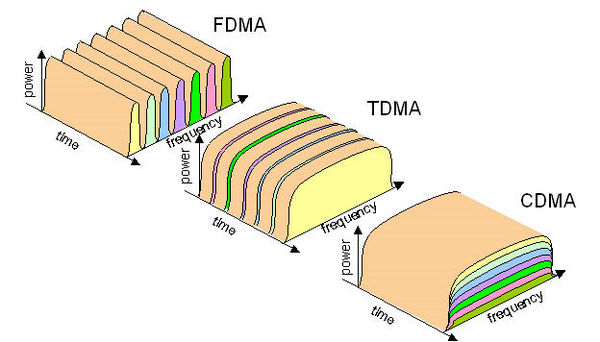
\includegraphics[width=\linewidth]{images/csma.jpg}
  \caption{Channel Multiplation}
  \label{fig:cmult}
\end{figure}

\paragraph{Multiplazione di spazio}
Le reti permettono di sfruttare la diversità spaziale del sistema per far coesistere più flussi di informazione in punti diversi. Questa possibilità può essere sfruttata per aumentare la capacità di una rete.\\
Tutte queste soluzioni possono essere applicate in modo predeterminato o in maniera statistica in modo da permettere una flessibilità relativa alla situazione.

\subsection{Commutazione di circuito}
Usata sin dagli albori della telefonia, usa le risorse disponibili per allocare un circuito (collegamento fisico) a ogni richiesta di servizio. Il circuito stabilito rimarrà ad uso esclusivo degli utenti per tutta la durata della loro connessione, le risorse verranno infatti rilasciate solo al termine della comunicazione. L'esempio principe è la rete telefonica.\\
I vantaggi principali sono:
\begin{itemize}
  \item Banda costante garantita.
  \item Ritardi costanti e ridotti.
  \item Trasparenza circuito (formati, velocità e protocolli).
\end{itemize}
Gli svantaggi invece:
\begin{itemize}
  \item Risorse dedicate.
  \item Buona efficenza solo per sorgenti continue.
  \item Tempo di apertura circuito.
  \item Tariffazione in base al tempo di allocazione.
\end{itemize}
Generalmente questa pratica risulta utile solo nel caso in cui il canale allocato risulti completamente sfruttato, altrimenti sarà sicuramente più vantaggioso lo smistamento.

\subsection{Commutazione di pacchetto}
L'idea principale di questo tipo di tecnologia è quella di non predeterminare l'allocazione, sopratutto per l'uso esclusivo da parte di due o più utenti. Questa tecnica può essere paragonata al sistema postale.\\
L'informazione da trasferire viene organizzata in unità dati (PDU) che comprendono informazioni di utente e protocollo.
\begin{itemize}
  \item \textbf{PDU:} Protocol Data Unit
  \item \textbf{PCI:} Protocol Control Information
  \item \textbf{SDU:} Service Data Unit
\end{itemize}
La PDU viene spesso chiamata pacchetto (packet) o datagram.\\
Ogni unità dati viene consegnata alla rete. Ogni nodo si occuperà di memorizzare il pacchetto, analizzare e determinare la destinazione del canale ed accodarlo per l'uscita. Questa tecnica prende il nome di \textbf{STORE \& FORWARD}.

\paragraph{Pacchetti}
Per poter funzionare questa tecnica ha bisogno di frazionare le informazioni in molti pacchetti ed essi potranno essere di dimensione fissa o variabile. In merito a questa soluzione vanno valutate alcune questioni riguardanti i vari ritardi nella trasmissione. Infatti in ogni canale in cui è trasmesso il nostro pacchetto subira un ritardo di TX (e di RX) in funzione della dimensione e della velocità della trasmissione ed un ritardo di propagazione in relazione alla lunghezza del canale.\\
Per ogni nodo invece avremo un ritardo di elaborazione ed un ritardo di accodamento (spesso trascurabili). Fortunatamente nella nostra comunicazione potremo sfruttare la parallelizzazione (pipeline) in modo da migliorare l'efficenza del nostro canale.\\
La dimensione dei pacchetti gioca un ruolo fondamentale nella trasmissione, pacchetti più brevi infatti favoriscono la parallelizzazione della trasmissione e diminuiscono la \% di errori, dovrò comunque tenere di conto che per ogni pacchetto avrò la necessità di un header.\\
I vantaggi principali di CAP:
\begin{itemize}
  \item Efficente utilizzo anceh con traffico intermittente.
  \item Possibilità di verifica del percorso.
  \item Conversioni possibili.
  \item Tariffazioni in funzione del traffico emesso.
\end{itemize}
Gli svantaggi sono invece:
\begin{itemize}
  \item Difficoltà ad ottenere garanzie di banda.
  \item Ogni nodo deve elaborare il pacchetto.
  \item Ritardi variabili.
\end{itemize}
Sostanzialmente la prima soluzione privilegia la qualità del servizio al singolo utente, la seconda invece l'efficenza complessiva della rete.\\

\paragraph{Modi di trasferimento}
In commutazione a pacchetto vi sono due principali modi per il trasferiemtno di informazioni. Quella datagram, descritta precedentemente, e quella a circuito virtuale.\\
La seconda soluzione si differenzia per la suddivisione in tre fasi:
\begin{enumerate}
  \item Apertura Connessione (segnalazione)
  \item Trasferiemento Dati
  \item Chiusura Connessione (segnalazione)
\end{enumerate}
Dopo aver stabilitò un'accordo tra i due interlocutori ed il fornitore i pacchetti seguiranno tutti lo stesso percorso a differenza del datagram dove i paccheti potrebbero tranquillamente seguire percorsi differenti. La soluzione a CV rimane comunque differente da quella a commutazione di circuito perchè non vengono allocate staticamente ed esclusivamente delle risorse.\\
Nel caso di datagram occorre identificare in ogni pacchetto SRC/DEST utilizzando identificatori globali. Nel caso di VC sarà sufficente individuare il percorso (sfruttando gli indicatori locali), le informazione SRC/DEST verrano utilizzate solo per stabilire il circuito. Questo tipi di circuiti può essere PVC (permanente) o SVC (commutato) ovvero create su richeista dell'utente trammite segnalazione della rete.
\begin{figure}[h!]
  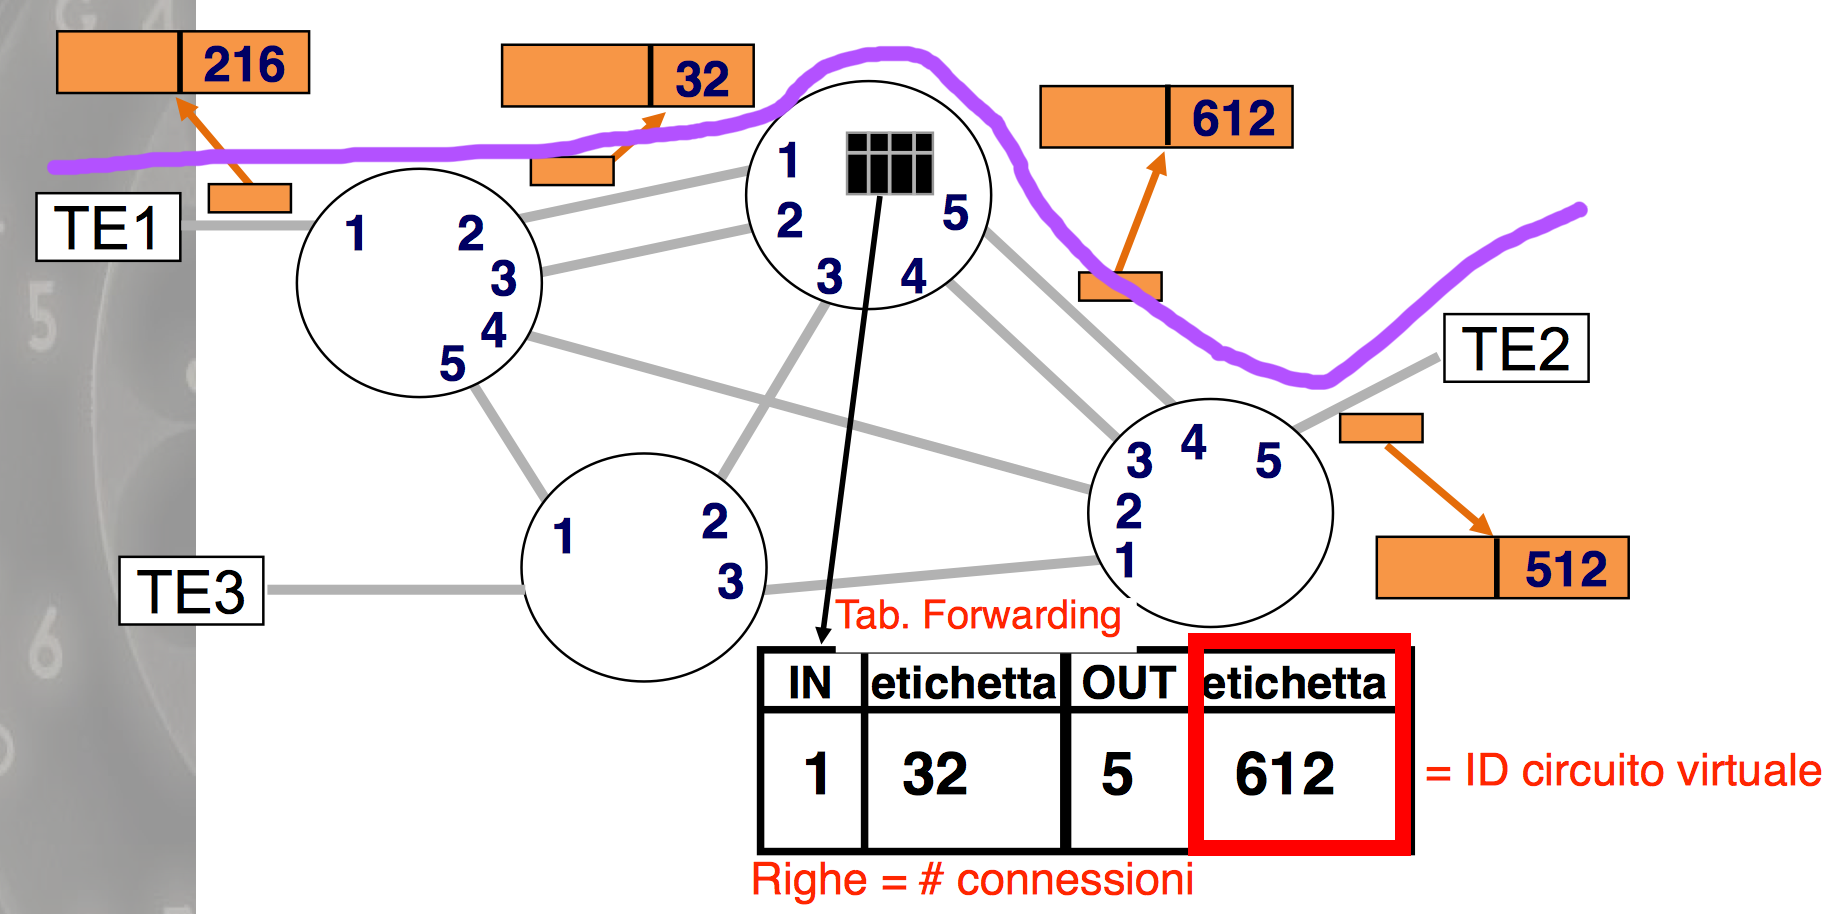
\includegraphics[width=\linewidth]{images/vc.png}
  \caption{Virtual Circuits}
  \label{fig:vc}
\end{figure} % 15 Dicembre 2016

\paragraph{Identificatori}
Un connessione su un canale è logicamente identificata trammite una etichetta, spesso una coppia di identificatori, questa soluzione permette di aggregare i flussi.\\

\subsection{Segnalazione}
Le segnalazioni possono essere di più tipologie, ci sono quelle di utente (scambio di informazioni tra utente e nodo), quelle internodali (con svambio di informazioni tra nodi), quelle associate al canale o quelle a canale comune.

\paragraph{Associata al canale}
Spesso usato nelle reti telefoniche stabilisce una corrispondenza biunivoca tra canale controllante (info segnalazione) e canale controllato (info utente). Nella versione fuori banda questa corrispondenza non c'è.

\paragraph{Canale comune}
Un canale di segnalazione controllo più canali di informazioni di utente mentre lavora a pacchetto.

\subsection{Tecniche di gestione}
Il network management consiste di diverse funzioni:
\begin{itemize}
  \item Configuration
  \item Performance
  \item Fault
  \item Security
  \item Accounting (tariffazione)
\end{itemize}

\subsection{QoS: \textit{Quality of Service}}
La qualità di un servizio offerto dipende dalla disponibilità di risorse nella rete e dalle tecniche di allocazione. L'analisi e il progetto di reti TLC si basa su modelli quantitativi in grado di stimare la qualità partendo da ipotesi relative alle risorse.\\
Supponendo un certa richiesta da soddisfare con un determinato numero di risorse si potrà determinare la qualità del servizio. Le sorgenti di informazione da trattare possono essere, come al solito, di tipo analogico o numeri, a velocità variabile o costante.\\
I principali indici di qualità sono:
\begin{itemize}
  \item Ritardi
  \item Velocità
  \item Probabilità errore
  \item Probabilità perdita
  \item Probabilità blocco
\end{itemize}
Un'esempio può essere la rete telefonica classica con una bassa latenza (qualceh decimo di secondo), una velocità di canale fino a 64 kb/s, una probabilità di errore non superiore a quale \% ed una scarsa probabilità di blocco.

\section{Architetture e Protocolli}
La comunicazione ha come unica pretesa la \textbf{COOPERAZIONE}. Le regole stabilite (convenzioni) che definiscono l'interazione tra elementi di una rete si chiamano protocolli.
\subsection{Protocolli}
``Sono la descrizione formale delle procedure adottate per assicurare la comunicazione tra due o più oggetti dello stello livello gerarchico.''\\
\rightline{{\rm --- \textbf{CCITT}}}
La definizione di protocolli prevede tre parti:
\begin{itemize}
  \item \textbf{Semantica}: Insieme di comandi e risposte.
  \item \textbf{Sintassi}: Struttura di comandi e risposte.
  \item \textbf{Temporizzazione}: Sequenze temporali di comandi e risposte.
\end{itemize}
Un'architettura di rete definisce il processo di comunicazione, le realazioni tra le parti coinvolte, le funzioni necessarie e le modalità organizzative.
\paragraph{Architetture stratificate}
Esse sono molto utili perchè ci garantiscono una semplicità di progetto, facilità di gestione, standardizzazione e separazione delle funzioni.

\subsection{Modello OSI}
Il modello OSI (Figure \ref{fig:osimodel}) (Open System Interconnection) è storicamente il primo modello a strati definito (1983) da ISO ec accettato da CCITT/ITU-T. Questo modello è la base di moltissime architettura ma non per questo devono rispettarlo nella sua interezza, internet ne usa solo alcuni strati per esempio.
\begin{figure}[!h]
  \centering
  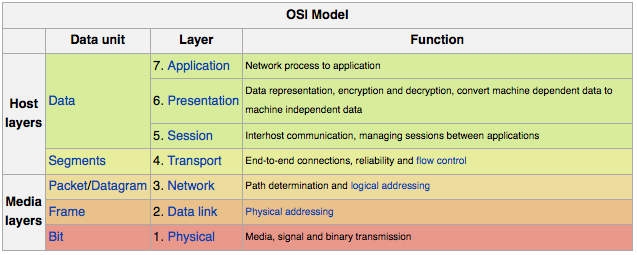
\includegraphics[width=\linewidth]{images/osimodel.jpg}
  \caption{OSI Model}
  \label{fig:osimodel}
\end{figure}
\paragraph{Implementazione}
A livello astratto possiamo immaginare una rete come composta da sistemi (terminali, nodi...) collegati tra loro da mezzi trasmissivi. Ogni sistema è composto da sottosistemi ed ognugno di essi realizza le funzioni del proprio strato tramite delle entità. Ogni strato fornisce servizi allo strato superiore usando servizi dello strato inferiore. Le entità sono gli elementi attivi di un sottosistema e svolgono le funzioni ed interagiscono all'interno di uno strato.\\
I sevizi possono essere:
\begin{itemize}
  \item \textbf{connection-oriented}: si stabilsice un'accordo preliminare tra rete e interlocutori, poi si trasferiscono i dati ed infine si rilascia la connessione.
  \item \textbf{connectionless}: i dati vengono immessi in rete senza accordi e sono trattati in modo indipendente.
\end{itemize}

\paragraph{SAP: Service Access Point}
La comunicazione tra due entità passa attraverso un punto di accesso al servizio (SAP).

\paragraph{Creazione PDU}
In un sistema a strati i dati utenti prensenti ad un N-esimo livello prendono il nome di N-SDU allora stesso modo anche la N-PCI che insieme andranno a formare la N-PDU. Ogni strato inferiore tratta la PDU di quello superiore come una busta chiusa a cui aggiungere solo la propria intestazione. Il sistema è paragonabile ad un palazzo dove al piano più alto scrivono la lettera e scendendo via via la imbusteranno, ci metteranno l'etichetta e verrà spedita. Il processo viene chiaramente svolto anche nel sistema ricevente ma in modo inverso.

\subsection{Livelli OSI}
Il sistema a strati definito precendetemente si divide in 7 livelli:
\begin{enumerate}
  \item \textbf{Physical Layer - Par. \ref{LV1}} :
  \begin{itemize}
    \item Fornisce i mezzi meccanici, fisici, funzionali e procedurali per attivare, mantenere e disattivare le connessioni fisiche.
    \item Trasferisce le cifre binarie scambiate tra le entità di strato collegamento.
    \item Definizione di codifiche di linea, connettori e livelli di tensione.
  \end{itemize}
  \item \textbf{Data link Layer - Par. \ref{LV2}}:
  \begin{itemize}
    \item Fornisce i mezzi funzionali per il trasferimento di informazioni tra le entità di strato rete e per fronteggiare malfunzionamenti di S1.
    \item Ha il compito di rilevare e recuperare gli errori, controllare il flusso e delimitare le unità dati.
  \end{itemize}
  \item \textbf{Network Layer - Par. \ref{LV3}}:
    \begin{itemize}
      \item Fornisce i mezzi per instaurare, mantenere ed abbattere le connessioni di rete tra entità dello strato trasporto.
      \item Gestisce instradamento, controllo di flusso/congestione e tariffazione.
    \end{itemize}
  \item \textbf{Transport Layer}:
    \begin{itemize}
      \item Colma le carenze di QoS dello strato rete.
      \item Controllo errore, sequenza e flusso.
      \item Multipla e demultipla le connessioni.
      \item Segmenta e ricompone i pacchetti.
    \end{itemize}
  \item \textbf{Session Layer}:
    \begin{itemize}
      \item Assicura alle entità di presentazione una connessione di sessione.
      \item Organizza la comunicazione tra enetità presentazione.
      \item Struttura lo scambio dati in modo da poterne avere una completa gestione
      \item Maschera le interruzioni del servizio di trasporto
      \item Spesso integrato nei livelli superiori.
    \end{itemize}
  \item \textbf{Presentation Layer}:
    \begin{itemize}
      \item Risolve i problemi di compatibilità nella rappresentazione dei dati.
      \item Risolve i problemi relativi alla trasformazione della sintasi dei dati.
      \item Può eventualmente fornire servizi di cifratura.
      \item Spesso integrato nei livelli superiori.
    \end{itemize}
    \item \textbf{Application Layer}:
      \begin{itemize}
        \item Fornisce ai processi applicativi i mezzi per accedere ad OSI.
        \item es: Mail, terminale virtuale, FTP, ecc...
      \end{itemize}
\end{enumerate} % 16 Dicembre 2016

\section{Protocolli a Finestra}
Sono i protocolli più frequenti nelle reti telematiche anche contemporanee. Usate in L2 ed L4. Si occupano principalmente di recupero degli errori di trasmissione, controllo del flusso e di sequenza.
\subsection{Errori di tramissione}
La trasmissione su qualsiasi canale non può mai essere esente da errori, la probabilità varia tra $10^-12$ (Optical Fiber) e $10^-3$ (Canale radio disturbato). Essendo però trasmessa una mole di dati dobbiamo comunque tenere in considerazione questi numeri e sviluppare tecniche per rilevare e correggere gli errori.
\paragraph{Codifica di canale} Per quanto un tecnica possa essere efficace comunque non ci potrà garantire una completa risoluzione dagli errori. Tra le più semplici (usate in molti ambiti diversi) ci sono:
\begin{itemize}
  \item \textbf{Parity BIT}: Aggiungo un numero che rappresenta se il numero di 1 (o 0) in una sequenza è pari (o dispari).
  \item \textbf{Codice a ripetizione}: Viene trasmessa più volte la stessa sequenza e si deciderà, la sequenza corretta, confrontandole.
  \item \textbf{Parity Righe/Colonne}: Analoga al parity bit ma la verifica viene fatta er ogni riga e per ogni colonna.
\end{itemize}
I bit di parità vengono sempre inseriti tra le informazioni di controllo (PCI) della PDU.
\paragraph{Correzione e Recupero}
Vi sono più soluzioni da adottare per l'utilizzo dei parity in base alla quanità.
\begin{itemize}
  \item \textbf{FEC} (Forward Error Correction): I tanti bit di parità vengono usati per cercare di corregge gli errori in ricezione senza la ritrasmissione del pacchetto.
  \item \textbf{ARQ} (Automatic Retransmission reQuest): I pochi bit di parità sono usati per rilevare gli errori e permettere al ricevitore di chiedere la ritrasmissione della PDU.
\end{itemize}
La tecnica migliore dipende dal contesto in cui andiamo ad operare.

\subsection{ARQ: \textit{Auto Retransmission}} \label{subsec:arq}
Questa tecnica sfrutta un controllo congiunto su errore, flusso e sequenza. Dovremo andare ad aggiungere un campo di numerazione (sequenza) all'interno delle PDU.\\
Vi sono 3 tecniche di implementazione:
\begin{enumerate}
  \item Stop \& Wait (Alternating Bit)
  \item Go back N
  \item Selective repeat
\end{enumerate}
Un'altro parametro da aggiungere prima di illustrare le tecniche è il \textbf{RTT} (Round Trip Time) una funzione del tempo che rappresenta il tempo necessario ad un pacchetto per essere inviato ed aver ricevuto la conferma, esso terrà conto dei ritardi introdotti da ogni elemento.

\paragraph{Semantica ACK}
Ogni protocollo ha la sua semantica per gli ACK, ovviamente TX ed RX devono preventivamente accordarsi su essa.\\
I più conosciuti sono:
\begin{itemize}
  \item \textbf{Cumulativo}: Si notifica la corretta ricezione di tutti i pacchetti con no. sequenza inferiore a quello specificato.\\
  AKC(n): ``\textit{Ho ricevuto tutto in sequenza fino ad n escluso}''
  \item \textbf{Selettivo}: Si notifica la corretta ricezione di un particolare pacchetto.\\
  ACK(n): ``\textit{Ho ricevuto il pacchetto n, ma non ti dono informazioni sui pacchetti precedenti o successivi}''
  \item \textbf{Negativo} (NAK): Si notifica la richiesta di ritrasmissione di un singolo pacchetto.\\
  NAK(n): ``\textit{Ritrasmetti il pacchetto n}''
  \item \textbf{Piggybacking}: Per risparmiare ACK, nel caso di comunicazioni bidirezionali, si permette di scrivere un riscontro ACK nella PDU di un'altro pacchetto.
\end{itemize}

\paragraph{STOP \& WAIT}
Questa algoritmo prevede semplicemente che il trasmettiroe dopo aver inviato la PDU resti in attesa (WAIT) dell'ACK di conferma da parte del ricevitore, nel caso qualcosa non vada secondo i piani si procederà alla ritrasmissione. Più precisamente prevede i seguenti step al \textbf{TRASMETTITORE}:
\begin{itemize}
  \item Invio PDU (e salvo copia)
  \item Avvio tempo di timeout
  \item Attendo ACK (acknowledgment)
  \item Se il $T_{out}$ scade ritrasmetto la PDU
\end{itemize}
Trasmettitore dopo aver ricevuto l'ACK:
\begin{itemize}
  \item Check correttezza ACK
  \item Check sequenza
  \item Se corretto, abilito l'invio della nuova PDU
\end{itemize}
Il \textbf{RICEVITORE} invece:
\begin{itemize}
  \item Check PDU
  \item Check sequenza
  \item Se corretta, invio ACK e consegno PDU a LV superiori
\end{itemize}
Durante l'utilizzo di questo algoritmo dobbiamo tenere in considerazione la numerazione delle PDU per due motivi. Primo sono indispensabili per il controllo di sequenza e secondo perchè la numerazione prevede un finito numero di bit. Può anche essere risolto con 1 solo bit ma la questione diventerebbe molto delicata, in generale avremo $2^n$ numeri prima di dover riprendere.\\
Altro fattore molto critico riguarda il tempo di timeout, la necessità è quella di scegliere un valore non troppo alto in modo da evitare inutili ritardi, ma allo stesso tempo non può essere troppo breve altrimenti la consegna dell'ACK potrebbe non avvenire in tempo.\\
Ulteriore improvement per S\&W potrebbe essere quello di utilizzare un time-to-live per ogni pacchetto.

\paragraph{Go back N}
La differenza principale rispetto al precedente è che non attenderemo ACK dopo ogni invio, la invieremo N PDU prima di rimanere in attesa delle conferme. Dato il multiplo invio dobbiamo introdurre il concetto di finestra.\\

\noindent\fbox{
  \parbox{\textwidth}{
  La \textbf{finestra TX} ($W_{T}$), rappresenta: ``\textit{La quantità massima di PDU che il trasmettitore è autorizzato ad inviare in rete senza aver ricevuto riscontro.}'', $W_{T}$ rappresenterà di conseguenza anche il massimo numero di PDU contemporaneamente presenti sul canale. La sua dimensione sarà $1<W_{T}\leq2^k$, il primo estremo non è compreso altrimenti sarebbe uguale a Stop \& Wait.\\
  La \textbf{finestra RX} ($W_{R}$) invece è: ``\textit{La sequenza di PDU che il ricevitore è disposto ad accettare e memorizzare.}'' ed è direttamente dipendente dalla memoria allocata alla ricezione.
  }
}\bigskip

Il TRASMETTITORE con finestra N:
\begin{itemize}
  \item Invia un numero di PDU corrispondenti alla $W_{T}$ facendo di ognugno la copia
  \item Avvia SOLO 1 contatore, per tutta le N*PDU, per il $T_{out}$
  \item Attende ACK
  \item Se scade $T_{out}$ ripeto la trasmissione di TUTTE le PDU
\end{itemize}
Il RICEVITORE invece:
\begin{itemize}
  \item Check PDU
  \item Check sequenza
  \item Se corretta, invio ACK e consegno PDU a LV superiori
\end{itemize}
Come per S\&W la $W_{R}$=1. Chiaramente la logica a TX sarà più complessa per via della finestra ampia.

\paragraph{Selective Repeat}
Possiamo definire questi algoritmi come uno sviluppo del precedente. In Go back N, il limite era dato dalla possibilità per il ricevitore di accettare solo PDU in sequenza. SR va proprio a compensare questo limite con $W_{R}>1$ solitamente di dimensioni pari. In generale $W_{T}+W_{R}\leq2^k$.\\
Può essere implementata in diversi modi con ACK Cumulativi o selettivi, timer su singole PDU o alla finestra e con vari comportamenti di TX ed RX. Si descrive il caso con ACK cumulativi e timer a finestra.
I compiti del TRASMETTITORE saranno:
\begin{itemize}
  \item Invia un numero di PDU corrispondenti alla $W_{T}$ facendo di ognugno la copia
  \item Avvia SOLO 1 contatore, per tutta le N*PDU, per il $T_{out}$
  \item Attende ACK
  \item Se scade $T_{out}$ ripeto la trasmissione di TUTTE le PDU
\end{itemize}
Il RICEVITORE invece:
\begin{itemize}
  \item Check PDU
  \item Check sequenza
  \item Se corretto
  \begin{itemize}
    \item \textbf{in sequenza} $\rightarrow$ consegna PDU a LV superiori
    \item \textbf{non in sequenza}:
    \begin{itemize}
      \item \textbf{in $W_{R}$} $\rightarrow$ Memorizzo
      \item \textbf{out $W_{R}$} $\rightarrow$ Scarto
    \end{itemize}
  \end{itemize}
  \item Invio ACK relativo all'ultima PDU in sequenza
\end{itemize}
Nel caso di singola perdita l'algoritmo si comporta come Go back N a livello di throughput ed occupazione del canale. Abbiamo vantaggi invece quando RTT $<$ $Tx_{Wr}$ perchè il nuovo ACK permetterà lo shift della finestra o in caso di perdite ripetute in quanto sarà necessaria una sola copia del pacchetto al RX. Se TX ritrasmettesse solo il primo pacchetto perso nella finestra ci sarebber un'ulteriore improvement come con gli ACK selettivi.

\section{Physical Layer - LV1} \label{LV1} % 18 Dicembre 2016
In questa sezione verranno presentati i mezzi trasmissivi dal punto di vista fisico e delle loro caratteristiche in ambito di utilizzo reale.
\subsection{Mezzi Trasmissivi}
I mezzi di trasmissione si distinguono grazie alle proprie caratteristiche. I mezzo ottimale presenterà resistenza, capacità parassite e impedenze basse, buona resistenza alla trazione, flessibilità e facilità di collegamento. Queste caratteristiche dipendono da moltissimi parametri come geometria, distanza, isolante, ecc...
\paragraph{Paramentri fisici}
Due importantissimi paramentri sono:
\begin{itemize}
  \item \textbf{Attenuazione}: Cresce linearmente, in dB, con la distanza e la $\sqrt{f}$
  \item \textbf{Diafonia o Cross-Talk}: Misura del disturbo introdotto da un cavo vicino. Cresce con la distanza fino a stabilizzarsi.
\end{itemize}
Si riporta una loro rappresentazione in figura \ref{fig:diaf_att}

\begin{figure}[!hp]
  \centering
  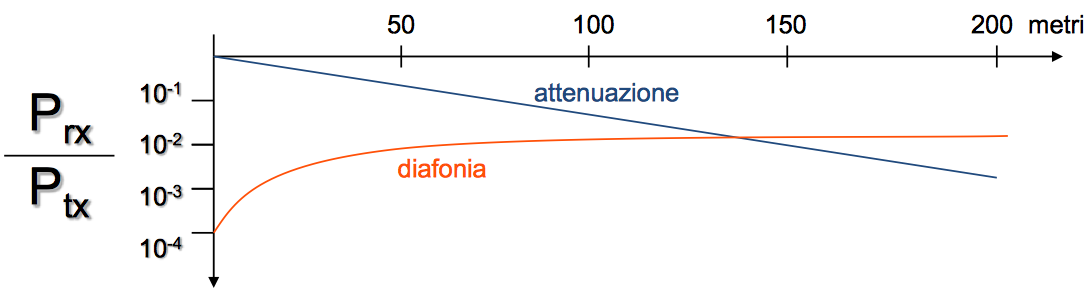
\includegraphics[width=\linewidth]{images/diaf_att.png}
  \caption{Rappresentazione Diafonia e Attenuazione}
  \label{fig:diaf_att}
\end{figure}
Le mezzi più comunemente utilizzati sono:
\begin{itemize}
  \item \textbf{Doppino} (Pair): Derivato dalla telefonia calssica e costituito da due fili di rame twisted per ridurre le interferenze elettromagnetiche. Economico, semplice e molto robusto. Usato nella sua versione non schermata UTP.
  \item \textbf{Coassiale}: Composto da un connettore centrale ed una o più calze di schermo per sfruttare la gabbia di Faraday e ridurre le interferenze. E' abbastanza costoso e non troppo semplice da installare ma più veloce del doppino. Usato molto con il connettore a T.
  \item \textbf{Fibra Ottica} (Optical fiber): Minuscolo e flessibile filo di vetro costituito da due parti (core e cladding) con diversi indici di rifrazione. Totale immunità a disturbi elettro/magnet, altissima capacità trasmissiva, bassissima attenuazione e dimensione/costi contenuti. Collegamenti non proprio semplici e poca flessibilità.
  \item \textbf{Canale Radio}: Notto anche some etere sfrutta la propagazione tra TX ed RX mediante l'uso di antenne. Garantisce di raggiungere grandi distanze (vedi satelliti). Molto dipendente dai fenomeni atmosferici e dagli ostacoli generanti riflessioni e rifrazioni (fading e shadowing).
\end{itemize}

\subsection{Codifiche di linea}
Per poter rappresentare segnali digitali mediante segnali digitali su mezzi elettrici e ottici abbiamo bisogno di codifice in modo da permettere a TX ed RX di comprendersi.

\paragraph{Unipolari}
Semplici, usano un livello di tensione per ogni valore, nulla per 0 e massima per 1. Il principale problema è legato alla continuita del segnale ed alla perdità di sincronismo in lunge trasmissioni con lo stesso simbolo.

\paragraph{Polari}
Sfruttano due livelli di tensione con polarità opposte in modo da ridurre la componente DC, vi sono 3 tipologie:
\begin{itemize}
  \item \textbf{NRZ}: Non c'è transizione da 0 da bit consecutivi.
  \item \textbf{RZ}: Tensione 0 tra due bit consecutivi.
  \item \textbf{Bifase}: Bit rappresentato da due livelli di tensione (es. Manchester).
\end{itemize}

\paragraph{Bipolari}
Chiamate anche AMI (\textit{Alternate Mark Inversion}) usano tensione nulla per 0 e due polarità opposte per 1 usate in alternativa. Permettono l'uso dei simboli ternari per ridurre i problemi di sincronismo con caratteri speciali di delimitazione e di scelta sulle parole di codice.

\paragraph{Modulazioni digitali}
Molto utilizzate per la rappresentazione di informazioni digitali mediante segnali analogici sui mezzi radio, ottici o elettrici dove l'informazioni viene impressa su di un segnale sinusoidale con variazioni di frequenza, fase o ampiezza per la distinzione dei segnali. % 19 Dicembre 2016

\subsection{Reti di Accesso}
L'utente si collega ad una rete di telecomunicazioni sfruttando sia la rete di accesso che quella di trasporto. La prima comprendo tutti gli apparati dall'utente al nodo di accesso, la seconda invece è costituita dai mezze appartenenti ad uno o più gestori di servizi di TLC destinati al transito su due nodi.\\
La gestione dell'ultimo miglio di rete, conosciuta anche come local loop, può essere gestita in più modi, con reti DSL, PON, HFC, ecc... Andremo ad analizzarle singolarmente.

\paragraph{DSL}
\textit{Digital Subscriber Line} è una famiglia di tecnologie in grado di fornire servizio dati ad alta velocità sulla rete. La più diffusa è quella asimmetrica (download maggiore di upload). In questo caso la vicinanza alla centrale è fondamentale.\\
L'accesso alla rete viene fatto attraverso un modem (MOdulatore DEModulatore) che ha il compito di trasformare il segnale da analogico a digitale e viceversa in modo da permettere la coesistenza del segnale dati e di quello voce per garantire la divisione in frequenza. La VDSL è una versione ``potenziata'' della ADSL in grado di garantire bitrate molto più elevati sfruttando bande di frequenza superiore.

\paragraph{PON}
\textit{Passive Optical Network} architettura per la connettività di last mile in fibra ottica senza componenti attivi. E' un'architettura poco diffusa in EU, molto invece in Asia, sostituisce direttamente FTTH ed integra VDSL.

\paragraph{HFC}
\textit{Hybrid Fiber Coax} sfruttano lo stesso meccaniscmo della TV via cavo, inzialmente erano unidirezionali, è strutturata sfruttando una topologia ad albero. Le differenze principali con ADSL sono legate alla condivisione degli apparati tra utenti della stessa zona residenzale, che ADSL sfrutta la rete telefonica senza richiesta di posa di cavi ad hoc a differenza di HFC. Il vantaggio principale è che non risente della distanza.\\

\paragraph{Cellulari}
Offrono servizi di voce e dati in mobilità. Il principio è quello di una copertura capillare tramite antenne con portata limitata. Si introducono i termini \textbf{Roaming} (rintracciabilità sul territorio) ed \textbf{Handover} (continuità di connessione nel passaggio tra celle).\\
Nel tempo sono passate alcune generazioni:
\begin{itemize}
  \item \textbf{1G}: Analogica, solo telefonia, grandi celle, bassa qualità ed efficenza.
  \item \textbf{2G} GSM: Digitale, FDMA/TDMA, celle contenute, criptata. Servizio dati con GPRS ed EDGE.
  \item \textbf{3G} UMTS: Servizi integrati dati e voce, FDMA/CDMA, celle stratificate, evoluta in HSPA.
  \item \textbf{4G} LTE: OFDMA con microcanali per brevi periodi, antenne MIMO.
\end{itemize}
\paragraph{Satellitari}
Ci son 3 tipologie di orbite, GEO usate per trasmissioni broadcast, MEO per GPS e LEO usati per telefonia satellitare.

\subsection{Reti di trasporto}
La rete di trasporto viene gestita da più operatori telefonici o dati (ISP) in competizione, alcuni sono anche proprietari delle infrastrutture (TIM), offrendo servizi o affittando gli apparati.\\
La trasmissione si è evoluta dalla rete telefonica tradizionale con multiplazione a divisione tempo.
\paragraph{Sincronizzazione}
Tutti i sistemi si sono evoluti dalla PDH (\textit{Plesiochronous Digital Hierarchy}) pensata per canali vocali, senza Store-and-Forward e con velocità limitate. Oggi si preferiscono infrastrutture sincrone come:
\begin{itemize}
  \item \textbf{SONET} \textit{Syncronous Optical NETwork}: Segnali otti multipli della velocità base.
  \item \textbf{SDH} \textit{Syncronous Digital Hierarchy}: Equivalente europeo di SONET.
  \item \textbf{STS} \textit{Syncronous Transport Signal}: Standard corrispondente per segnali elettrici.
\end{itemize}
Per questioni di affidabilità vengono preferite strutture ad anello. Lo schema di divisone solitamente è temporale (TDM) ed ogni trama include una PCI con informazioni per la sincronizzazione, canali di servizio e gestione guasti.

\section{Data Link Layer - LV2} \label{LV2}
Le principali funzioni di questo strato, sfruttate poi dal superiore sono:
\begin{itemize}
  \item Delimitazione di trama
  \item Multiplazione
  \item Indirizzamento locale
  \item Rilevazione errore
  \item Controllo di flusso sull'interfaccia
  \item Correzione errore
\end{itemize}
Derivano dal protocollo SDLC utilizzato inizialmente da IBM SNA, standardizzato poi da ISO come HDLC. Da esso derivano molti altri protocolli come LAPB, LAPD, ecc... Si è poi aggiunto un sottostrato MAC nelle reti locali.\\
I protocolli di LV2 sono usati sia dalle \textbf{reti pubbliche} per gestire le connessioni tra utente e nodo, sia nelle \textbf{reti private} per connettere tra di loro apparati in ambienti circoscritti.
\paragraph{Trasferimento}
Un caratteristica comune ai due tipi di rete rimane la PDU composta come in tabella:
\begin{center}
  \begin{tabular}{ |c||c|c|c|c|c|c| }
    \hline
    \textbf{Dato} & 01111110 & Indirizzo & Controllo & Dati & CRC & 01111110 \\
    \hline
    \textbf{Size} & 8 & 8 & 8/16 & $\geq 0$ & 16 & 8\\
    \hline
  \end{tabular}
\end{center}
Una considerazione da fare riguardo il flag di controllo che è importante non confondere con parte di dati, per farlo si usano tecniche come Bit o Byte Stuffing. Esse sfruttano un singolo bit dopo ogni sequenza di 5 uni tranne che nel flag, oppure una sequenza di escape da scartare prima del flag.

\subsection{PPP: \textit{Point to Point Protocol}}
Utilizzato nei collegamenti telefonici o ADSL. Le caratteristiche speciali di questo protoccolo sono:
\begin{itemize}
  \item Negoziazine dell'indirizzi di LV1
  \item Trasparenza del contenuto
  \item Semplicità
  \item Rilevazione senza recupero degli errori
\end{itemize}
I campi della PDU sono simili a quelli classici con flag, address (compatibilità HDLC), control (compatibilità HDLC) e protocol (procotollo di livello superiore a cui consegnare i dati).\\
Questo standard inizia dallo stato di dead, cercherà di stabilire una connessione e nel caso di successo configurerà la rete per essere utilizzata. Dopo l'eventuale autenticazione interviene NCP che definirà le modalità di trasferimento e negozierà l'assegnazione di un indirizzo.

\subsection{Frame Relay}
Standard per costruire reti a pacchetto con circuiti virtuali (vedi figura \ref{fig:vc}) su scala geografica. Il nome è la tecnologia, mentre il protocollo è LAPF. Ancora usato per collegare di nodi degli ISP.\\
LAPF è suddiviso in due parti, DL$-$CORE (utilizzato da tutti i nodi della rete) DL$-$CONTROL (utilizzato solo dal mittente e dal destinatario).

\subsection{ATM: \textit{Asynchronous Trasfer Mode}}
Rete integrata nata durante l'evoluzione di ISDN, chiamata B-ISDN. Anche essa è una rete a pacchetto con servizi di VC su scala geografica.\\
 Il servizio sarebbe stato ottimo ma non è molto diffuso a livello utente per la necessità di sostituire tutti gli apparati esistenti. I vataggi di questa tecnologia riguardano principalmente le velocità elevate, bassa latenza ed uso di PDU di dimensione fissa (53 byte, 48 B di dati). Interessante l'analisi dell''intestazione della cella, composta da:
 \begin{itemize}
   \item \textbf{GFC - 4b}: Contiene informazioni riguardanti il numero di celle immettibili nella rete.
   \item \textbf{VPI - 8/12b}: Percorso definito tra più commutatori ATM.
   \item \textbf{VCI - 16b}: Singolo circuito interno a VP.
   \item \textbf{PT - 3b}: Classifica il tipo di informazione contenuta nel payload. Ha siginificato in AAL5.
   \item \textbf{CLP - 1b}: Cell Loss Priority.
   \item \textbf{HEC - 8b}: Header Error Code.
 \end{itemize}
La struttura AAL (\textit{ATM Adaption Layer}) integra il trasporto ATM per offrire differenti servizi ai livelli superiori. In particolare viene usato AAL5 usato per gestire la segmentazione di PDU a LV3.

\subsection{LLC: \textit{Logical Link Protocol}}
Il LV2 viene suddiviso in 2 sottolivelli, LLC (derivato da HDLC) e MAC (Medium Access Controll).\\
E' un protocollo standard (ISO 8802/2 e IEEE 802.2) di caratteristiche tipo:
\begin{itemize}
  \item Orientato al byte.
  \item Senza delimitatori (demandato al MAC).
  \item Non check errori (non esiste il campo CRC).
  \item PDU con indirizzi SRC e DEST.
  \item PDU di dimensione variabile.
\end{itemize}

\section{Protocolli Reti Locali - LAN}
La rete locale solitamente è una ridotta estensione geografica dove abbiamo necessità di trasmissioni simultane tra più utenti, per questo motivo è necessario gestire la condivisone del canale.\\
Una possibile soluzione è quella di convisione rigida del canale o per frequenza, codice o tempo. Il problema è che un'allocazione statica porterebbe a grosse limitazioni vista la natura del traffico, devo quindi emulare una multiplazione statistica. Vi sono 3 principali famiglie, a contesa (Ethernet, Wi$-$Fi), ad accesso ordinato (Token Ring o bus ed FDDI) o con slot a prenotazione (DQDB).
\subsection{Accesso Casuale}
In questa soluzione quando un nodo deve trasmettere lo fa alla velocità R senza coordinarsi con altri nodi, con possibilità di collisione.\\
Il primo esempio è \textbf{Aloha} (di \textit{Norm Abramson} 1970). Soluzione semplice senza sincronizzazione, la trasmissione viene iniziata in qualunque istante, la conferma viene ricevuta su un canale separato, nel caso non venga ricevuta dopo un tempo di timeout ritrasmetto dopo un tempo casuale (in caso di ulteriore collisione raddopio il tempo casuale). Chiaramente con questa soluzione la probabilità di collisione è elevata.\\
Lo \textbf{Slotted Aloha} invece divide il tempo in slot, solo ad inzio slot potrà essere avviata una trasmissione, se si verifica collisione ritrasmetto sempre con il criterio di prima. L'efficenza non è molto alta (18-37\%) e non è nemmeno stabile. La distribuzione viene rappresentata in figura \ref{fig:eff_lan}

\begin{figure}[!hp]
  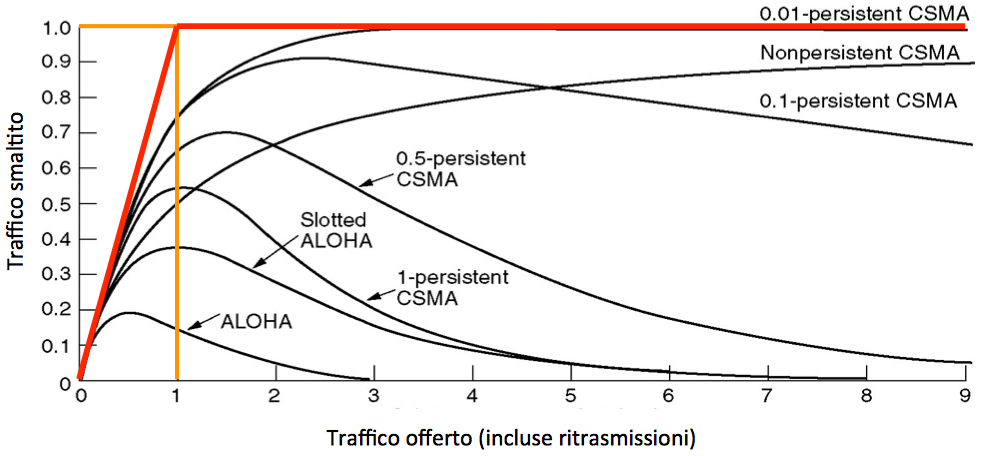
\includegraphics[width=\textwidth]{images/eff_lan.png}
  \caption{Efficenza reti LAN (Linea ROSSA ideale)}
  \label{fig:eff_lan}
\end{figure}

\subsection{CSMA: \textit{Carrier Sense Multiple Access}}
La bassa efficenza di Aloha è dovuta dall'accesso casuale ai canali. Per aumentare il throughput e diminuire le collisioni posso eseguire semplicemente una verifica della liberà o no del canale.\\
Vengono utilizzate le seguenti strategie di ritardo trasmissione:
\begin{itemize}
  \item \textbf{1-persistent}: Aspetto che il canale si liberi e trasmetto immediatamente.
  \item \textbf{non-persistent}: Riprovo a sentire il canale dopo un tempo casuale, se libero ritrasmetto.
  \item \textbf{p-persistent}: Aspetto che il canale si liberi e trasmetto con probabilità p o rimando la trasmissione con probabilità (1-p).
\end{itemize}
Anche in questa soluzione si avranno collisioni, sono inevitabili, perchè direttamente correlati al tempo di propagazione sul canale. Un possibile modo per compensare queste mancanze si ha con le versioni CD (collision detection) o CA (collision avoidance).
\paragraph{Collision Detection}
La stazione monitora il canale durante la trasmissione:
\begin{itemize}
  \item Se sente sola la propria prosegue.
  \item Se sente collisione, interrompe la propria.
\end{itemize}
Devo comunque considerare un margine di errore, se una trasmissione termina pochi istanti dopo che un'altra è iniziata potrei non rilevare la collisione. Le performance di questa soluzione migliorano su reti piccole, su reti piccole rispetto alla dimensione della trama e con velocità di trasmissione bassa. Si preferisce la soluzione 1-persistent perchè migliore a basso carico, non è facile la gestione delle priorità. Soluzione adottata in \textbf{Ethernet}.
\paragraph{Collision Avoidance}
Non è possibile usare la versione CD su canali radio, per tanto preferisco prevenire le collisioni.\\
La procedura è strutturata in questo modo:
\begin{itemize}
  \item Ascolto per un tempo DIFS e se rimane libero per tutto il tempo inzio trasmissione.
  \item Se durante questo spazio DIFS il canale si occupa, avvio un timer di \textit{backoff} e finito esseo rieseguirò il punto precedente.
\end{itemize}
La ricezione invece prevede la verifica della correttezza di trama per l'invio di un ACK ovviamente, nel caso in cui TX non ricevesse ACK ripartirà la procedura di trasmissione. Le collissioni si possono comunque verificare ma con una probabilità minore. Questo procollo viene usato nelle reti \textbf{WiFi 802.11}.

\section{Standard Reti Locali - LAN}
L'inizio della standardizzazione di questi protocolli è degli anni \`80 dal progetto IEEE 802, con definizioni da 802.1 (Itroduzione all'internet working di LAN), fino ad 802.17 (resilient packet ring). Le principali funzioni di LV2 sono già state presentate in nel capitolo \ref{LV2}.\\
Introduciamo ora il concetto di indirrizi LLC, ovvero di indirizzi che permetto la multiplazione di più protocolli di strato superiore, e di indirizzi MAC i quali permettono di identificare la scheda (TX o RX) trai i nodi della LAN.
\subsection{Indirizzi MAC}
Sono numeri di 6 byte, inizialmente scritti in una ROM della scheda, ora modificabili anche via software, sono composti di due parti. I primi 3 byte MS sono un lotto di indirizzi assegnati al costruttore (Organization Unique ld.), gli ultimi 3 rappresentano una numerazione progressica interna decisa dal costruttore. \textit{Esempio:} \textbf{EC:22:80}:07:9A:4D \textit{è una scheda DLink.}\\
Possono essere di 3 tipi:
\begin{itemize}
  \item \textbf{UNICAST}: Singola stazione.
  \item \textbf{MULTICAST}: Gruppi di stazioni.
  \begin{itemize}
    \item \textbf{Solicitation}: Richiesta di servizio ad un gruppo multicast.
    \item \textbf{Advertisement}: Periodica diffusione di informazioni di appartenenza ad un gruppo M.
  \end{itemize}
  \item \textbf{BROADCAST}: Riferiti a tutte le stazioni.
\end{itemize}
Una volta ricevuto un pacchetto la scheda si occuperà di verificare se il MAC coincide, in caso positivo la invierà a livelli superiori, in caso non lo sia verra scartato (possibile eventuale override software).

\subsection{Ethernet}
\paragraph{Ethernet vs IEEE 802.3}
Le differenze tra questi due standard sono solo di tipo tecnico relative al livello MAC e fisico, vedi figura \ref{fig:eth} e \ref{fig:ieee8023} .
\begin{figure}[!hbpt]
  \centering
  \begin{minipage}{.45\textwidth}
    \centering
    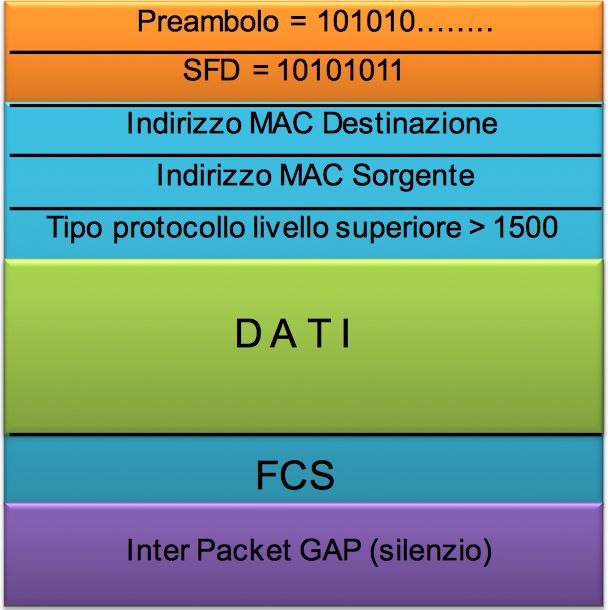
\includegraphics[width=\linewidth]{images/eth.png}
    \caption{Ethernet}
    \label{fig:eth}
  \end{minipage}\hfill
  \begin{minipage}{.45\textwidth}
    \centering
    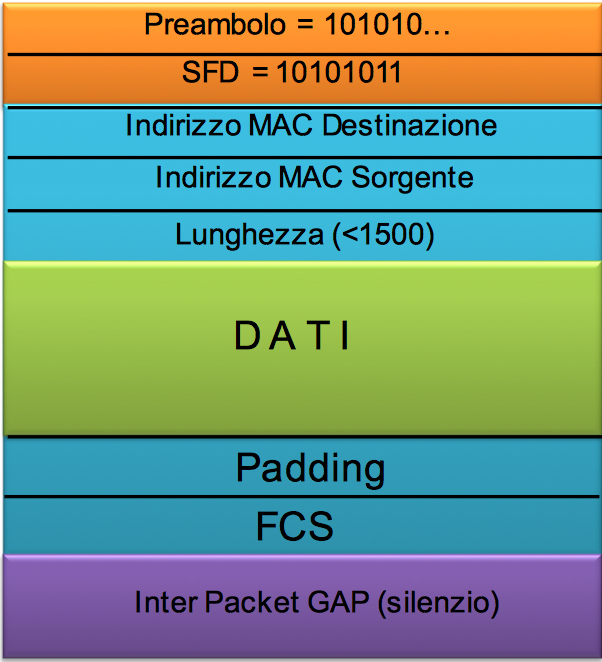
\includegraphics[width=\linewidth]{images/ieee8023.png}
    \caption{IEEE 802.3}
    \label{fig:ieee8023}
  \end{minipage}\hfill
\end{figure}
Se stazioni sono nello stesso dominio di collisione, il tempo minimo di trasmissione di una trama non può essere inferiore al massimo RTT. Da questa affermazione deriva che la velocità di trasmissione e le dimensioni della rete determinano la lunghezza minima della trama.\\
Le principali caratteristiche di questa rete sono:
\begin{itemize}
  \item Non caricare troppo per mantenere buona efficenza.
  \item Semplice e totalmente distribuito.
  \item Non adatto ad applicativi real-time.
  \item Piccoli ritardi a basso carico
  \item Molto diffuso.
  \item Nessuna conferma di ricezione.
  \item No priorità.
\end{itemize}
\subsection{Apparati}
Le reti locali sono sempre più efficenti, veloci ed affidabili. Si cerca di aumentarne sempre di più estensione, numero di utenti e sicurezza.
\paragraph{HUB}
Sono apparati multiporta che operano a LV1 (paragrafo \ref{LV1}) sono quindi passivi, non riconosce le trame e non separa di domini di collisione.
\paragraph{Switch}
Sono apparati multiporta operanti a LV2 (paragrafo \ref{LV2}) attivi con funzioni di store-and-forward (riconosce trame) in grado di garantire prestazioni superiori agli hub.\\
Il vataggio principale rispetto al primo dispositivo è quello di separare i domini di collisione, creandoli ad hoc per ogni connessione punto-punto, eliminando così di fatto le collisioni (CSMA/CD non più necessario) e trasformando ETH in un protocollo ``framing'' di LV2.\\
Questi dispositivi non dovrebbero modificare la struttura della rete, è necessario però che ogni apparato abbiamo un indirizzo di LV2 unico all'interno della LAN estesa. Il funzionamento è basato sulla conoscenza topologica della rete per tanto vi son 3 tecniche di switching:
\begin{itemize}
  \item \textbf{Address Learning}: Per ogni trama viene letto e memorizzato l'indirizzo MAC sorgente ed asseganto alla porta.
  \item \textbf{Frame Forwarding}: Dopo aver ricevuto un packet cerca se la destinazione è presente nel database, se la trova invia alla porta precisa altrimetni invia a tutti tranne a quella sorgente.
  \item \textbf{Spanning Tree}: Genera un'albero logico in modo da eliminare anelli, abitando solo alcune porte.
\end{itemize}
\paragraph{Vantaggi di interconnesione}
Questo ampliamento degli apparati di rete genera molti vantaggi:
\begin{itemize}
  \item Partizionamento della rete in K reti locali.
  \item Diminuzione o rimozione di collisione.
  \item Trasforma la rete da classica a commutazione di pacchetto.
  \item Gestibilità e sicurezza.
\end{itemize}
\paragraph{VLAN: Virtual LAN}
Sono LAN costituite da host fisicamente collegati allo stesso segmento di rete ma logicamente partizionati in LAN separate. E' un costrutto di LV2 che deve quindi essere supportato dallo switch.

\subsection{WiFi}
\paragraph{WiFi vs IEEE 802.11}
``WiFi'' è una certificazione di interoperabilità e aderenza allo standar, rilasciata da una associazione di produttoti (WiFi Alliance). La definizione di IEEE invece è il nome di una famiglia di standar che copre la tecnologia delle reti locali wireless dal punto di vista fisico, MAC, interconnessione e sicurezza.\\
La rete può essere creata senza struttura WiFi Direct (comunicazione diretta tra terminali) o tramite AP (Access Point), eventualmente collegato ad internet, funzionalmente analogo ad uno switch a livello MAC.
\paragraph{Strato Fisico}
802.11 lavora su bande NON LICENZIATE esse infatti sono condivise dal moltissimi strumenti come Bluetooth, Cordless, forni MW, ecc... Le frequenze in questione sono 2.4 GHz (14 channel) e 5 GHz (23 channel).
\paragraph{Strato MAC}
A questo livello la struttura si basa su DCF (\textit{Distributed Coordination Function}) direttamente derivato da CSMA/CA. Le differenze sono legate alla contesa, per una stazione, del possesso del canale. Essendo stazioni half-duplex il ricevitore dovra confermare con ACK la ricezione. Datenere in considerazione la collisione in caso di terminale nascosto, risolvibile però con handshaking, invianto una piccola trama contenente la durata del trasferimento.
% TERMINE ARGOMENTI DI STRUTTURA - 20 Dicembre 2016
% ------------------------------------------------------------------------------------ %

% ARGOMENTI PROTOCOLLI - 20 Dicembre 2016

\section{Network Layer - LV3} \label{LV3}
\subsection{Introduzione}
Il livello 2 (\ref{LV2}) presenta alcuni problemi come la bassa efficenza nella gestione dei collegamenti, ecc... Il livello 3 cerca di compensare alcune di queste carenze.\\
Questo livello di occupa di trasportare i pacchetti dal TX ad RX, di incapsulare i pacchetti (lato TX) e di consegnarli al LV4 (lato RX). Questo livello è presente in ogni tipo di dispositivo che sia esso Host o Router.\\
Le due principali funzioni di questo strato sono quella di \textbf{routing} e di \textbf{forwarding}. La prima, per analogia, equivale a ``\textit{Pianificare un viaggio dalla sorgente alla destinazione}'' mentre la seconda a ``\textit{L'attraversamento di ogni singolo incrocio}''.

\subsection{Datagram o VC}
La soluzione con datagram fornisce un servizio di networks \textit{connectionless} mentre i virtual-circuit ne forniscono uno \textit{connection}.\\
Ricampitolando le principali differenze sono:
\begin{itemize}
  \item \textbf{Datagram}:
  \begin{itemize}
    \item Scambi tra host molto elastici.
    \item Molte tipologie (alcuni problemi di uniformità).
    \item Terminali molto SMART, \textbf{complexity at ``edge''}.
  \end{itemize}
  \item \textbf{VC}:
  \begin{itemize}
    \item Evoluta dalla telefonia.
    \item Precisa temporizzazione per garantire il servizio.
    \item Terminali ``stupidi'', \textbf{complexity ``inside''}.
  \end{itemize}
\end{itemize}

\subsection{IP Datagram}
Il LV3 contribuisce alla formazione del pacchetto da trasferire per una totale comprensione. I campi del datagram (IPv4), rappresentati in figura \ref{fig:ipdata}, sono:
\begin{itemize}
  \item \textbf{Versione}: IPv4 o IPv6.
  \item \textbf{Header Lenght}: Dimensione dell'header in 32 B.
  \item \textbf{Type of Service}: Tipo di dato, usato per prioritizzare il traffico.
  \item \textbf{Length}: Lunghezza complessiva del datagram.
  \item \textbf{16-bit ID}: Utilizzato per frammentazione e riassemblaggio.
  \item \textbf{Flags}: Utilizzato per frammentazione e riassemblaggio.
  \item \textbf{Fragment Offset}: Utilizzato per frammentazione e riassemblaggio.
  \item \textbf{TTL}: Numero di rimanenti passaggi (hops).
  \item \textbf{Upper Layer}: Protocollo di livello superiore per la consegna del payload.
  \item \textbf{Header Checksum}
  \item \textbf{32 bit IP SRC}: Indirizzo IP di sorgente.
  \item \textbf{32 bit IP DEST}: Indirizzo IP della destinazione.
  \item \textbf{Options}: Timestamp, record route, list of router, ecc... Non sempre presente.
  \item \textbf{Payload}: Dati di pacchetto, tipicamente segmenti TCP o UDP.
\end{itemize}

\begin{figure}[!hp]
  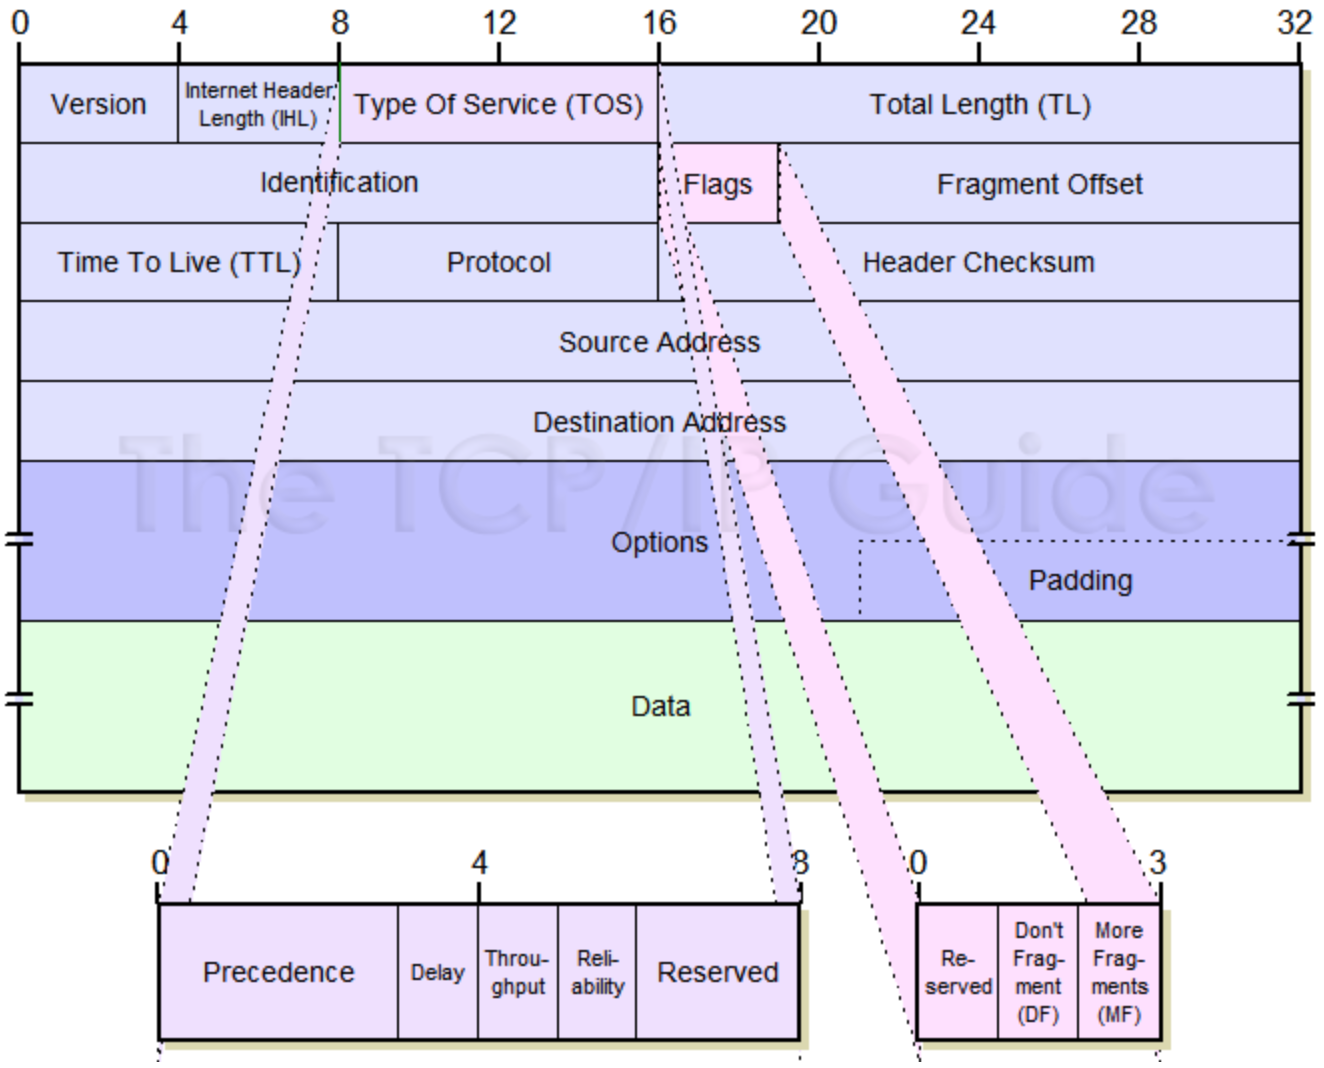
\includegraphics[width=\textwidth]{images/ipheader.png}
  \caption{IPv4 Datagram}
  \label{fig:ipdata}
\end{figure}

Tutto questo header si aggiunge ai quelli dei precedenti e successivi. % 24 Dicembre 2016

% 5 Gennaio 2017 - 14:32
\paragraph{Frammentazione} Nel datagram IP è presente una sezione di flag per la frammentazione essa è necessaria al fine di ricostruire correttamente il pacchetto. Questo flag è costituito da una terna di bit:
\begin{enumerate}
  \item Riservato (sempre a 0).
  \item = 1 se NON frammentato.
  \item = 1 se presenti ulteriori frammenti.
\end{enumerate}

\subsection{IP Addressing} % 5 Gennaio 2017
L'indirizzo IP, come detto precedentemente, si riferisce direttamente all'interfaccia dell'host e non all'host stesso, questo perchè esso potrebbe avere interfacce multiple. Le interfacce invece rappresentano il collegamento fisico tra host e router (sia che esso sia wireless o no). Un esempio di indirizzo IP:
\begin{equation}
  \begin{gathered}
    223.1.1.1 = 11011111|00000001|00000001|00000001
    \label{eq:ipv4bit}
  \end{gathered}
\end{equation}
Come avvenga la connessione tra due interfacce non è interesse di LV3.\\
L'indirizzo IP è costituito da due parti, la prima di NETWORK (spesso chiamata erroneamente SUBNET) costituita dai bit più significativi e da una parte di HOST costituita dai rimanenti. Host multipli sullo stesso NETWORK devono porter senza l'utilizzo di un router questo perchè risultano essere sulal stessa rete IP, quando invece parliamo di due network differenti allora necessitiamo di un router che ci permetta l'interconnessione fra più reti. In una visione molto pratica possiamo quasi dire che la rete IP sia sul ``filo stesso'' vista la sua natura.
\paragraph{Indirizzi Riservati} All'interno di una qualsiasi struttura IP si presentano una moltitudine di indirizzi, è importante però che alcuni di questi rimangano riservati per questione che vedremo successivamente. Sicuramente ogni rete IP necessità un per il nome della rete e di uno di broadcast.

\subsection{Protocollo ARP} % 5 Gennaio 2017
La rete LAN è il principale apparato sfruttato per le comunicazioni tra host, ogni interfaccia deve necessariamente possedere un proprio indirizzo IP ed un indirizzo MAC unico. Chiaramente questo porta, da parte di un router, a dover conoscere le destinazioni per la corretta consegna dei pacchetti.\\
Le informazioni necessarie alla corretta consegna di un pacchetto sono molte e non sempre sono tutte già disponibili, sopratutto all'avvio della rete, per questo viene in aiuto il protocollo \textbf{ARP} (\textit{Address Resolution Protocol}) in grado i recuperare queste informazioni mancanti. Il funzionamento della procedura ARP è il seguente:
\begin{enumerate}
  \item A vuole inviare a B, ma non ha nella sua ARP table il MAC dell'interfaccia di B.
  \item A invia un \textbf{ARP request} (\textbf{broadcast}, inviata a tutti gli host) contenente l'indirizzo IP di B e FF:FF:FF:FF:FF:FF come indirizzo MAC.
  \item Una volta ricevuta da B, essa risponde \textbf{ARP reply} con il proprio MAC address ad A (\textbf{unicast}, invio diretto all'host scelto).
  \item A riceve il pacchetto ed aggiunge l'informazione del MAC di B nella propria ARP table fino a scadenza.
\end{enumerate}
E' importante ricordarsi che i pacchetti ARP non sono pacchetti IP, ma sono parte del paylod di pacchetti di LV2.

\subsection{Indirizzamento LAN esterne} % 5 Gennaio 2017
Una delle caratteristiche più interessanti delle reti di calcolatori è proprio la comunicazione tra di esse, abbiamo visto come comunicare internamente ad una singola rete, ma se volessimo comunicare con una LAN differente invece?\\
La procedura non è molto differente sarà necessario un'ulteriore passaggio attraverso un router.
\begin{enumerate}
  \item A crea il datagram per B (nell'altra rete IP) utilizzando però come IP e MAC di destinazione non quelli di B, ma del proprio R (router, default gateaway) che sarà eventualmente connesso alle altre reti IP.
  \item R rimuove le informazioni MAC e passa a livello IP.
  \item R crea il nuovo datagram da inviare mettendo come informazioni si SRC quelle della proprio interfaccia collegata alla rete IP di B e come informazioni di dest quelle dell'host B.
  \item B riceve il pacchetto e lo gestisce.
\end{enumerate}
Questa procedura non prevede l'utilizzo di ARP.

\subsection{Classi IP} \label{subsec:ipclass} % 5 Gennaio 2017
Abbiamo priam parlato delle due parti presenti a livello IP (network ed host) ma non di come distinguerle! Vi sono tre possibili soluzioni:
\begin{itemize}
  \item \textbf{Classful addressing}: Divisione statica delle due parti, tre possibili dimensioni di rete IP, non sfrutta il concetto di subnetting ed è poco flessibile:
  \begin{itemize}
    \item \textbf{Class A} (128 net): $10.0.0.0\rightarrow10.255.255.255$ - PFL: 8
    \item \textbf{Class B} (16K net): $172.16.0.0\rightarrow172.31.255.255$ - PFL: 12
    \item \textbf{Class C} (2M net): $192.168.0.0\rightarrow192.168.255.255$ - PFL: 16
    \item \textbf{Class D}: Multicast Address
    \item \textbf{Class E}: Reserved for Future Use
  \end{itemize}
  \item \textbf{Subnetting}: Parte dalla struttura a classi completa definendo però reti più piccole chiamate ``subnet'' (VLSM).
  \item \textbf{Classless addressing}: Rimuove completamente il concetto di classi IP (CIDR).
\end{itemize}
Uno dei principali problemi di IPv4 è lo spreco di indirizzi IP per questo son stati creati due meccanismi in grado di migliorarne l'utilizzo sprecando meno indirizzi possibili e sono VLSM e CIDR.

\subsection{Configurazione Host} \label{subsec:hostconfig} % 5 Gennaio 2017
Un device per poter essere collegato alla rete recessiterà di alcuni paramentri fondamentali, senza i quali non potra sfruttare al pieno le possibilità della rete o eventualmente nessuna. Le 3 informazioni che deve ricevere, è possibile sia invia automatica DHCP, sia in via manuale) sono:
\begin{itemize}
  \item \textbf{Indirizzo IP}
  \item \textbf{Netmask}: Necessaria per valutare la la posizione di un'altro host, se interna o esterna alla proprio rete IP.
  \item \textbf{Default Gateaway}: Il primo passo per una comunicazione indiretta (verso un'altra rete IP).
  \item \textbf{Server DNS}: Solitamente due indirizzi necessari alla traduzione degli indirizzi testuali (\textit{es. google.it}), vedi capitolo \ref{sec:dns}.
\end{itemize}
L'host ha il compito di verificare se la connessione che vuole instaurare è interna o meno al suo network.
\paragraph{Check IP} Per svolgere questa operazione esegue un doppio confronto, calcola il risultato di un'operazione di AND tra il proprio IP e la propria netmask e di un'altra operazione di AND ma tra l'IP di destinazione e la propria netmask, se questi due risultati saranno uguali allora significa che la comunicazione sarà diretta, ovvero che i due host risiedono sulla stessa rete IP, nel caso i due risultati differiscano la comunicazione sara indiretta.

\subsection{Routing IP}
La comunicazione all'interno di una rete prevede la definizione di ``strade'' percorribili al fine di poter comunicare tra host, queste tabelle son definite all'interno dei routers e possono essere di 3 tipi:
\begin{itemize}
  \item \textbf{Dirette}: Strade direttamente linkate al router.
  \item \textbf{Statiche}: Le strade per altri network vengono definite manualmente.
  \item \textbf{Dinamiche}: Definizione automatica delle strade tramite protocolli di routing e ICMP redirect.
\end{itemize}

\subsection{DHCP: \textit{Dynamic Host Configuration Protocol}} % 5 Gennaio 2017
Tra i campi necessari introdotti nel capitolo \ref{subsec:hostconfig} abbiamo parlato dell'indirizzo IP. Vi sono due possibili soluzioni per ottenere, o viene definito manualmente (Static IP), o viene assegnato da un protocollo ``plug-and-play'' chiamato DHCP.\\
L'iter è abbastanza semplice ed avviene alla connessione di un nuovo host (vedi figura \ref{fig:dhcp}):
\begin{enumerate}
  \item \textbf{Discover}: Il client appena connesso invia un messaggio broadcast (IP DEST 255.255.255.255) senza IP SRC.
  \item \textbf{Offer}: Il server DHCP invia un pacchetto broadcast con l'indirizzo IP che vorrebbe assegnare al nuovo client. Pacchetto con lifetime $\neq$ 0.
  \item \textbf{Request}: Il client risponde accettando l'indirizzo che gli viene assegnato (nel pacchetto non viene ancora messo come IP SRC). Pacchetto con lifetime $\neq$ 0.
  \item \textbf{ACK}: Il server invia l'ultimo pacchetto, sempre broadcast, dove conferma l'assegnazione definitiva dell'IP in questione. Pacchetto con lifetime $\neq$ 0.
\end{enumerate}

\begin{figure}[!hbpt]
  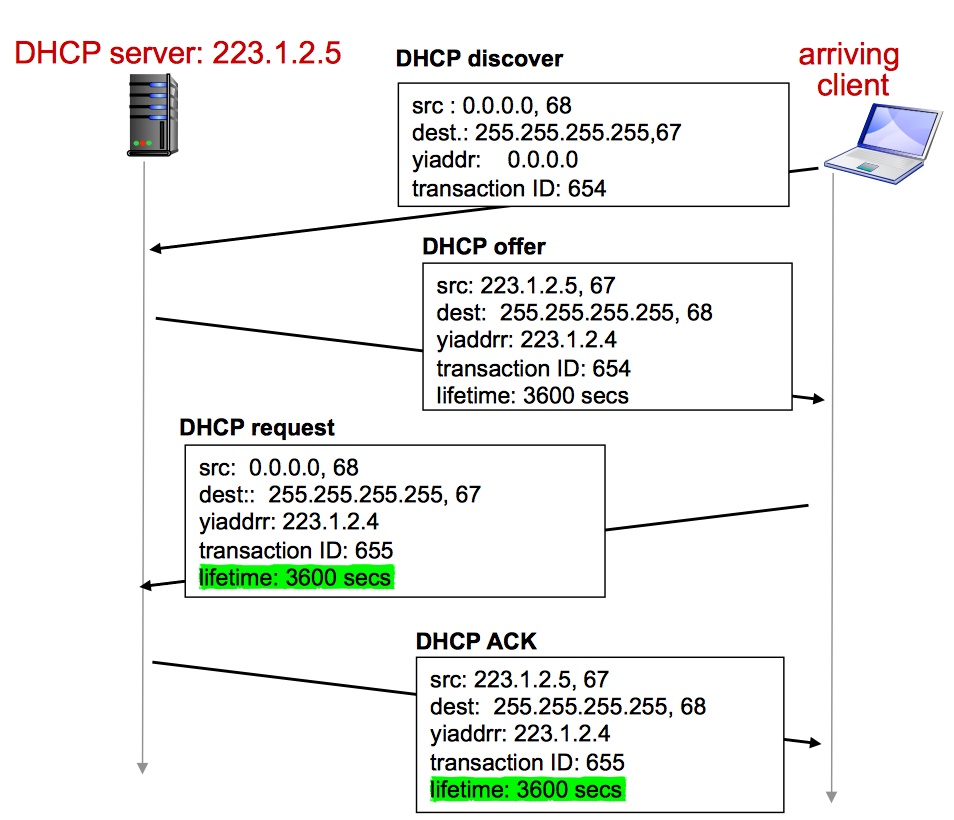
\includegraphics[width=\textwidth]{images/dhcp.png}
  \caption{DHCP Flow}
  \label{fig:dhcp}
\end{figure}

L'indirizzo assegnato, salvo diverse impostazioni da parte dell'amministratore di rete, non è permanente, viene infatti definito un \textbf{tempo di lease}. A metà di questo tempo, il DHCP, cerca di rinnovare l'indirizzo assegnato, se la procedura avviene con successo allora viene riavviato il cronometro del tempo di lease, altrimenti l'indirizzo viene segnato come libero dal server.\\
Il ruolo del server DHCP non si limita solamente all'assegnazione dell'indirizzo IP, si occupa di comunicare anche l'indirizzo del router (\textit{first-hop address o default gateaway}), il nome e l'indirizzo dei server DNS e la netmask.\\
Si potrebbe talvolta sentir parlare di DHCP Service in quanto spesso non è un hardware dedicato ma viene installato su altre apparecchiature, tipo router.

\paragraph{Last hope} Nel caso in cui non sia stata definita nessuna informazione in modo statico, nel caso in cui il server DHCP non risponda o non esista, il nostro dispositivo tenterà una connessione STATELESS scegliendo un indirizzo a caso in 168.254.x.y/16, verificando prima se ARP request a quell'indirizzo non risponde, ed autoassegnandoselo.

\subsection{IP Pubblici}
Ad oggi la questione IP pubblici è molto delicata infatti non sono più disponibili spazi, questo è dovuto alle limitazioni della struttura IPv4 creata più di 40 anni fa quando non si sapeva nemmeno a cosa si sarebbe andati in contro. L'aumento esponenziale dei dispositivi IoT sicuramente non ha agevolato la cosa se ci aggiungiamo la transizione per nulla semplice ad IPv6 si capisce la situazione in cui siamo.\\
L'ente che si occupa di assegnare i blocchi di IP agli operatori si chiama ICANN (\textit{Internet Corporation for Assigned Names and Numbers}) ed ha lo scopo di allocare indirizzi, gestire i DNS, assegnare i nomi ai domini e risolvere le dispute.

\paragraph{Allocazione} L'allocazione di questi indirizzi avviene a livello geografico scalare, vengono asseganti blocchi continentali, dove esistono ulteriori enti di divisione, si passa poi alle divisioni nazionali tra operatori ed infine agli utenti finali.

\subsection{NAT: \textit{Network Address Translation}} %  13 Gennaio 2017
Il crescente numero di device ha portato alla carenza di indirizzi IP per l'indirizzamento dei dispositivi. Per questo motivo è stato necessario trovare una soluzione al problema.\\
Nella attuale struttura di indirizzamento vi sono alcuni indirizzi ``privati'' ovvero non annunciati pubblicamente sulla rete e di conseguenza non raggiungibili, vengono definite nello stesso modo delle reti classful (paragrafo \ref{subsec:ipclass}) ma comunque valide in CIDR.
\paragraph{Traduzione} Spesso il concetto di NAT viene frainteso, il ruolo degli home gateaway ricopre molti ambiti tra cui NAT e PATH. Il NAT ha il compito di tradurre gli indirizzi della rete locale con un singolo indirizzo, rappresentante la rete, in tutta internet.
\paragraph{Funzionamento} Il NAT ha il compito di rappresentare la nostra rete locale nel ``mondo internet'' per fare questo traduce tutti i pacchetti in uscita, costituiti da una porta sorgente e da un indirizzo IP interno alla rete, con un indirizzo rappresentante la nostra rete e con una differente porta. Esattamente allo stesso modo, al arrivo di un pacchetto nella nostra rete, il NAT si occuperà di recapitare al giusto host della rete locale il pacchetto. Il procedimento si basa sull'utilizzo di una tabella (\textit{NAT Translation Table}) contenente le varie entri di porta ed indirizzo ``interni'' e porta ``esterna''.
\paragraph{Problema NAT} A livello pratico tutti i dispositivi di una rete vengo visti da internet come un singolo indirizzo IP, di conseguenza non si può indirizzare precisamente un host all'interno di una rete, per farlo bisogna gestire il tutto in modo opportuno, allocando staticamente una tabella per il forwarding oppure usando relaying server.
La prima soluzione è abbastanza semplice e non necessità di essere spiegata.\\
Servizi come Skype necessitano una connessione alla rete per funzionare ma l'utente chiamante non avrebbe modo di connettersi a chi vuole senza conoscerne la sua porta, per tanto vengono sfruttare i relaying server. Con la seguente procedura:
\begin{itemize}
  \item NAT e client1 stabiliscono una connessione con il realy server.
  \item Client2 si connette anch'esso al relay server.
  \item Il realy server farà da ponte tra le due connessioni permettendo ai due client di comunicare correttamente.
\end{itemize}



\subsection{ICMP}

\subsection{IPv6}

\subsection{Algoritmi di Routing}


%----------------------------------------------------------------------------------------
\section{DNS: \textit{Domain Name System}} \label{sec:dns} % 6 Gennaio 2017
Questo capitolo si occuperà di descrivi i DNS e la loro utilità nelle operazioni di tutti i giorni.

\subsection{Introduzione} % 6 Gennaio 2017
Il servizio DNS è stato implementato per permettere all'utente di utilizzare nomi più ``human readable'' riespetto ad indirizzi IP numerici.\\
Il servizio in questione è costituito da batabase distribuiti geograficamente (in tutto il mondo) in modo hierarchico ed opera a livello applicativo (LV.7). I suoi compiti sono la traduzione degli indirizzi testuali (es. \textit{google.it}) in indirizzi IP classici (es. 172.217.23.67), l'aliasing, l'aliasing per i mail server e la distribuzione del carico (multi-IP per singolo nome).

\subsection{Struttura} % 6 Gennaio 2017
La struttura dei DNS è molto importante al fine di gestire correttamente ed in modo efficente il traffico in entrata e uscita da essi.\\
Quando un'utente chiedere di accedere ad un indirizzo come \textit{www.amazon.com} la procedura che si attiva non è per nulla banale (questa è la procedura completa, non considera caching):
\begin{enumerate}
  \item Il client interroga il \textbf{root server} per chiedere informazioni sul DNS \textbf{.com}.
  \item Il client interroga il DNS \textbf{.com} per chiedere informazioni sul DNS \textbf{amazon.com}.
  \item Il client interroga il DNS \textbf{amazon.com} per richiedere l'indirizzo IP di \textbf{www.amazon.com}.
\end{enumerate}
Riepilogando:

\begin{figure}[!hbpt]
  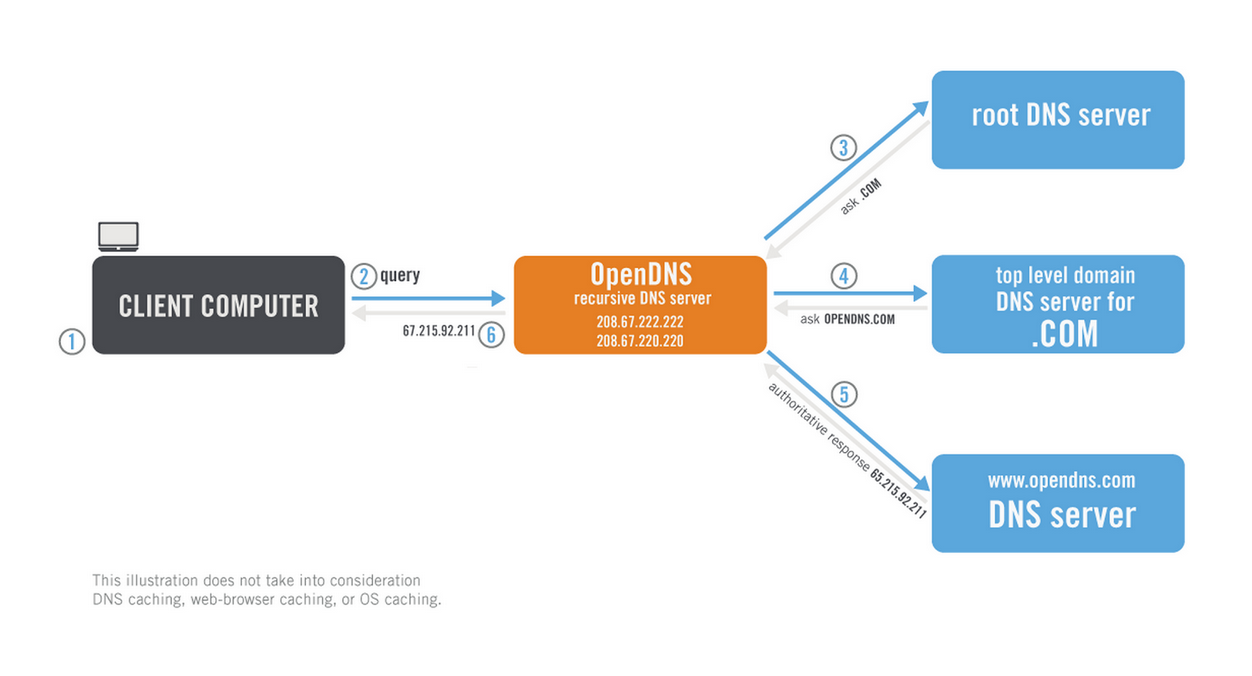
\includegraphics[width=\textwidth]{images/dnsflow.png}
  \caption{DNS Flow}
  \label{fig:dnsflow}
\end{figure}

I \textbf{Root DNS Servers} sono 13 ed hanno il compito della prima gestione di risoluzione DNS. Fortunamente non vengono interrogati ogni volta dal singolo utente ma vengono richiesti qualora un \textit{local name server} non riesca a risolvere automaticamente un nome. Questi server infatti possono contattare gli \textit{authoritative name server} per mappare e restituire il percorso al local server richiedente informazioni.

\subsection{Tipologie} % 6 Gennaio 2017
Esistono diversi tipi di DNS e non tutti svolgono lo stesso compito all'interno della rete.
Vi sono:
\begin{itemize}
  \item \textbf{TLD}: \textit{top-level domain}
  \begin{itemize}
    \item Commerciali: .com, .org, .net, .jobs
    \item Nazionali: .it, .us, .fr, .uk
    \item Educativi: .edu
  \end{itemize}
  \item \textbf{Authoritative}: Di proprietà di aziende, ISP, ecc... ed hanno il commpito di fornire IP per mappare gli host nella rete.
  \item \textbf{Local}: Non fanno per forza parte della struttura gerarchica e sono solitamente di ISP piccoli, università o simili. Chiamati spesso DEFAULT name server.
\end{itemize}

\subsection{Risoluzione Nomi}\label{subsec:dnsresolution} % 6 Gennaio 2017
Vi sono due strategie principali per la risoluzioni dei nomi, una iterativa ed una ricorsiva.\\
La strategia \textbf{iterativa} si basa sull'interrogazione, da parte dell'host che chiede la risoluzione di un nome, del \textit{local DNS server}, una volta partita la prima richiesta sarà il local ad eseguire tutti i passaggi, andando a chiedere al root, al TLD, ed infine al authoritative che ci risponderà con l'indirizzo; solo a quel punto il local DNS potrà restituirci l'indirizzo. Vedi figura \ref{fig:itedns}.\\
Nel caso della strategia \textbf{ricorsiva} invece, una volta fatta la richiesta al local, verrà fatta la prima interrogazione al root, sarà poi il root stesso a fare la richiesta al TLD, di conseguenza il TLD la farà all'authoritative, una volta ricevuta risponda ogni server si occuperà di rispondere al livello superiore fino ad arrivare all'host. Vedi figura \ref{fig:recdns}.

\begin{figure}[!hbpt]
  \centering
  \begin{minipage}{.45\textwidth}
    \centering
    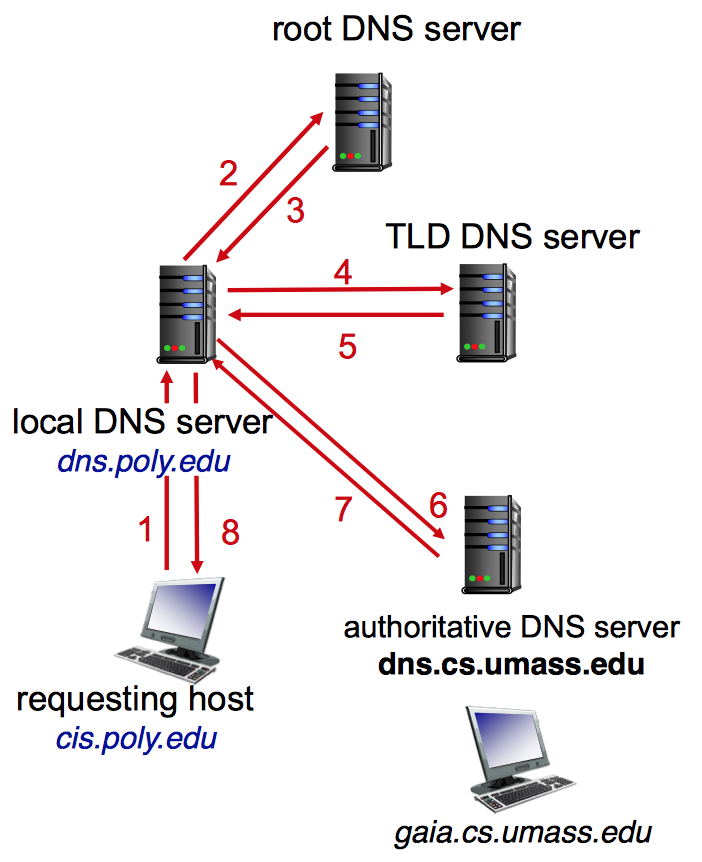
\includegraphics[width=\linewidth]{images/itedns.png}
    \caption{Risoluzione nomi iterativa}
    \label{fig:itedns}
  \end{minipage}\hfill
  \begin{minipage}{.45\textwidth}
    \centering
    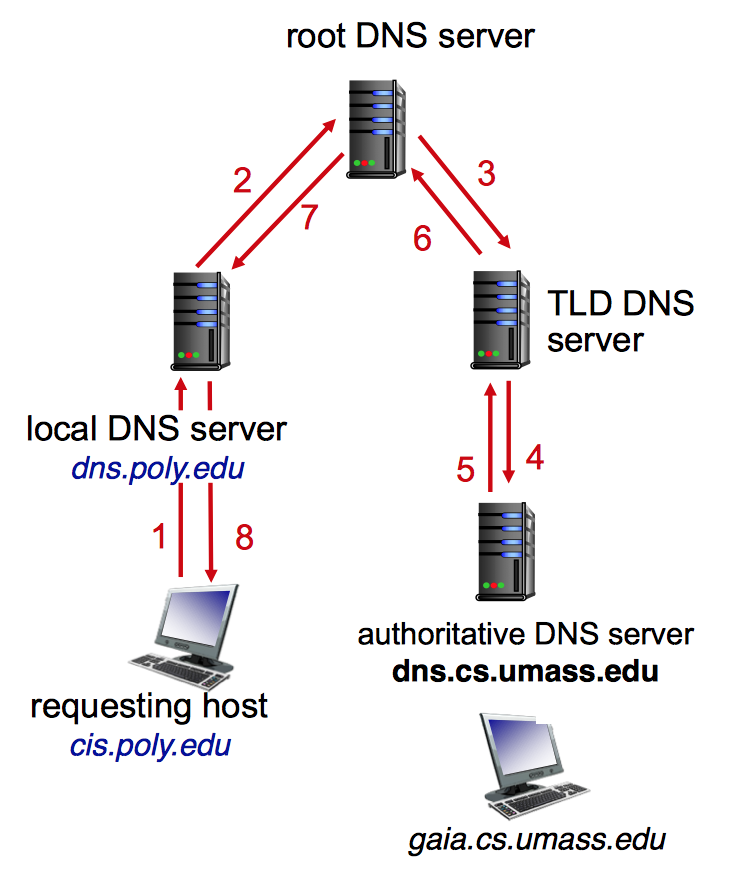
\includegraphics[width=\linewidth]{images/recdns.png}
    \caption{Risoluzione nomi ricorsiva}
    \label{fig:recdns}
  \end{minipage}\hfill
\end{figure}

\subsection{Caching} % 6 Gennaio 2017
Fortunatamente la procedura descritta nel capitolo precedente non viene iterata tutte le volte altrimenti difficilmente si riuscirebbe a gestire il traffico generalo al giorno d'oggi. Infatti vengono usati moltissimi meccanismi di caching in modo da minimizzare il numero di ricerche.\\
Ogni qualvolta un host richiede la risoluzione di un nome viene svolta la procedura del capitolo \ref{subsec:dnsresolution} danno una risposta all'utente ma salvando anche la risposta nella propria in cache in modo da non dover effettuare nuovamente la ricerca nel caso in cui quella risoluzione venga nuovamente richiesta, spesso infatti i server TLD vengono cached nei local. Questo algoritmo potrebbe portare a risoluzioni non funzionanti, in caso di cambiamenti di topologia esterna, quindi dopo un certo TTL (\textit{Time To Live}) vengono rimosse le entry dalla cache e viene rieffettuata la ricerca.

\paragraph{Record} Come detto precedentemente il servizio DNS non si occupa solo di risolvere da Nome $\rightarrow$ Indirizzo, ma di gestire anche alias e server mail. Proprio per questo nella cache del DNS vanno tenute anche informazioni riguardanti la tipologia di record, il tipo, ecc... nel formato:
\begin{equation}
  \begin{gathered}
    \textbf{RR}(name, value, type, ttl)
  \end{gathered}
\end{equation}
Vengono categorizzata per TYPE =
\begin{itemize}
  \item \textbf{A}:
  \begin{itemize}
    \item name: Nome host
    \item value: Indirizzo IP
  \end{itemize}
  \item \textbf{NS}:
  \begin{itemize}
    \item name: Dominio
    \item value: Nome del server authoritative per quel dominio
  \end{itemize}
  \item \textbf{CNAME}:
  \begin{itemize}
    \item name: Alias per quale nome canonico (reale) [es. ibm.com]
    \item value: Nome canonico [es. servereast.backup2.ibm.com]
  \end{itemize}
  \item \textbf{MX}:
  \begin{itemize}
    \item name: Nome
    \item value: Mail server associato al nome
  \end{itemize}
\end{itemize}

\section{Transport Layer - LV4} \label{LV4} % 6 Gennaio 2017
\subsection{Introduzione} % 6 Gennaio 2017
Il livello 4 di occupa di gestire le comunicazioni logiche tra applicativi presenti su host differenti. Come tutti gli altri livelli sfrutta il precedente (LV3) per fornire a sua volta funzioni al livello successivo (LV5).\\
Questo protocollo di trasmissione lavora nei singoli terminali (to edge), nel lato sender si occupa di segmentare i messaggi del livello application per passarli a livello network, mentre, lato receiver, si occupa di prendere i pacchetti frammentati dal network layer e riassemblarli per l'application. In poche parole il LV3 si occupa della \textit{logica di comunicazione tra due host}, mentre il LV3 si occupa della \textit{logica di comunicazione tra processi applicativi}.\\
Esistono due protocolli di trasmissione, TCP (resistente ed ordinato) ed UDP (debole e disordinato), che verrano successivamente analizzati.

\subsection{Multiplexing} \label{subsec:mpx} % 6 Gennaio 2017
Un necessario passaggio durante le comunicazioni tra calcolatori è sicuramente la consegna e l'aggregazione dei pacchetti in arrivo ed uscita. Questo step è necessario per via della moltitudine di applicativi attivi contemporaneamente su ogni host. Lato sender significa gestire dati da più applicativi, aggiungerli l'header del corrente livello e passarli al livello network. Lato receiver invece significa leggere l'header, del pacchetto appena ricevuto dal livello network, e consegnarlo all'applicativo corretto.

\paragraph{Flow} La consegna/raggruppamento si basa su due ulteriori campi, diversi da tutti i precedenti visti, la \textit{source} e \textit{destination ports}. Da qui poi derivano due possibili tecniche di mux/demux:
\begin{itemize}
  \item \textbf{Connectionless} (UDP): Usa IP e \#Port di destinazione e sorgente, riferendosi direttamente al socket, per la gestione della comunicazione. [\textit{fig. }\ref{fig:udp_mux}]
  \item \textbf{Connection-oriented} (TCP): Usa tutti e 4 i campi IP e \#Port sia di destinazione che di sorgente per capire a quale socket consegnare i pacchetti. Permette di gestire più connessioni simultanee. [\textit{fig. }\ref{fig:tcp_mux}]
\end{itemize}

\begin{figure}[!hbpt]
  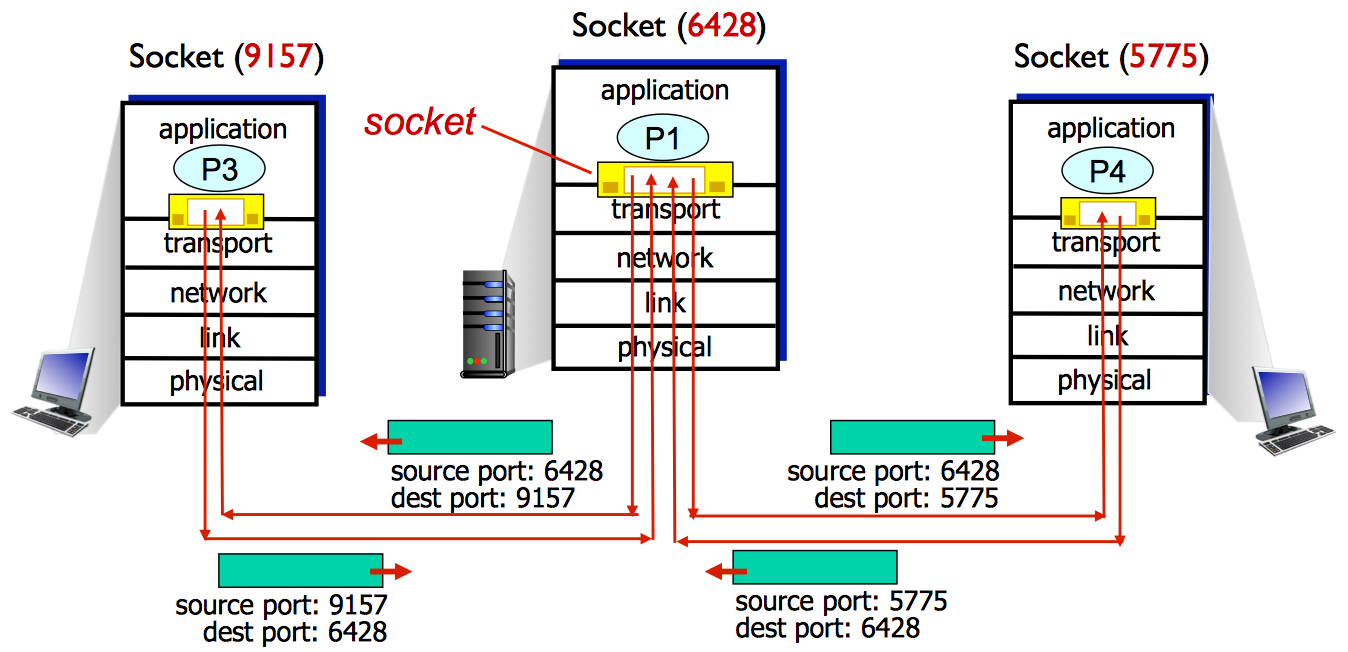
\includegraphics[width=\textwidth]{images/udp_mux.png}
  \caption{UDP Muxltiplexing/Demultiplezing Flow}
  \label{fig:udp_mux}

  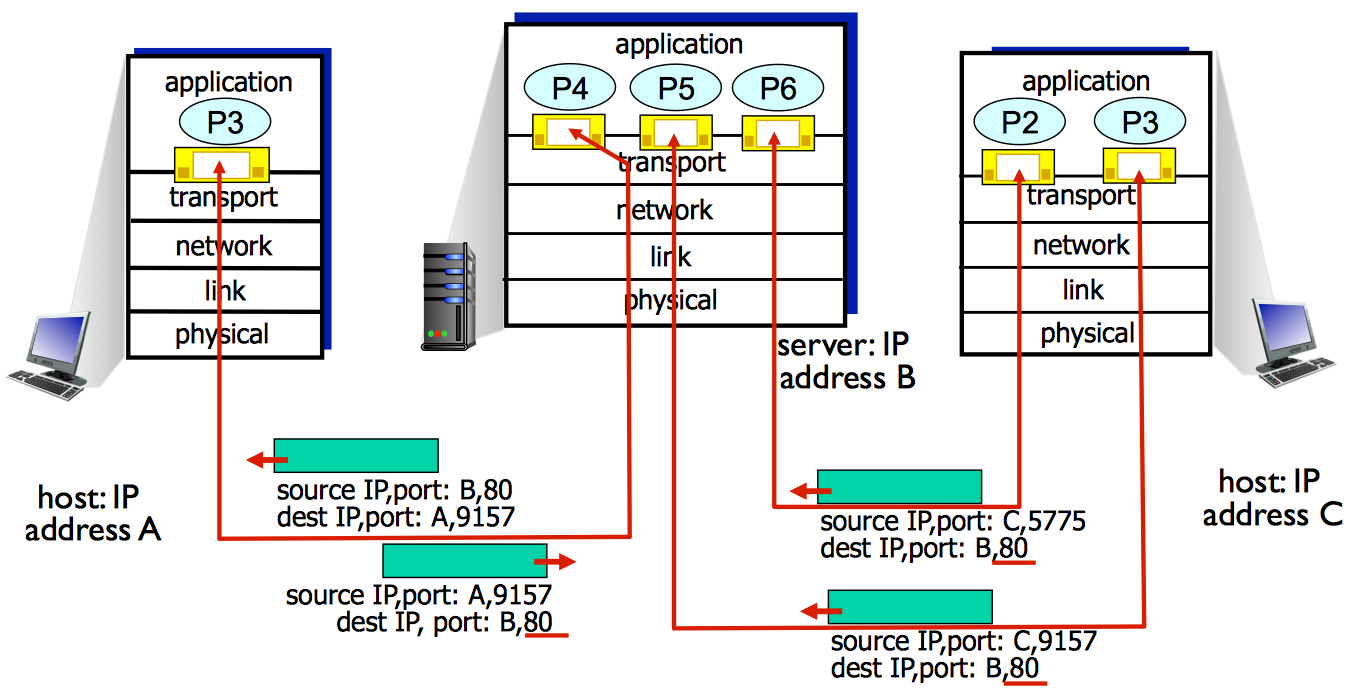
\includegraphics[width=\textwidth]{images/tcp_mux.png}
  \caption{TCP Muxltiplexing/Demultiplezing Flow}
  \label{fig:tcp_mux}
\end{figure}

La comunicazione, utilizzando le porte, prevede che il sender sappia a quale porta inviare i pacchetti. Alcune di queste porte son state definite dagli enti (SSH 22, FTP 21, HTTP 80, HTTPS 8080, ecc...), altre vengono scelte dalle app direttamente in modo casuale oppure possono essere definite dall'utente manualmente.

\subsection{UDP: \textit{User Datagram Protocol} [RFC 768]} % 7 Gennaio 2017
Il protocollo UDP è attualmente molto utilizzato, insieme a TCP, a livello trasporto per le comunicazioni. Bisogna però fare alcune considerazioni in merito a questo protocollo in modo da poterlo utilizzare correttamente.\\

\paragraph{Caratteristiche} Questo tipo di protocollo viene definito \textit{connectionless} ovvero che, come definito in \ref{subsec:mpx}, non prevede nessun tipo di handshaking prima di avviare la comunicazione tra TX ed RX ed ogni pacchetto risulta essere gestito indipendentemente dagli altri pacchetti anche se provenienti dalla stessa comunicazione (spesso disordinati). Il non utilizzo di \textit{handshaking} porta sicuramente a problemi di connessione infatti il pacchetto potrebbe essere stato inviato dove non c'è nessuno in ascolto, potrebbe non essere nemmeno uscito dalla rete e tante altre cose da tenere in considerazione.\\
Essnedo una connessione poco ``affidabile'' viene utilizzata in tutti quei campi in cui la perdita non provocherebbe grossi danni come streaming multimediale, DNS, DHCP, ecc...\\
Tutte questo considerazioni non vanno interpretate come negative infatti questo protocollo essendo molto semplice e facile da gestire permette meno congestione, non necessità di connessione quindi niente ritardi ed ha un header più piccolo.

\paragraph{Header} I campi aggiunti da questo protocollo sono:
\begin{center}
\begin{tabular}{ |c||c|c|c|c|c| }
 \hline
 \textbf{Field} & SRC Port\# & DEST Port\# & Length & Checksum & Payload \\
 \hline
 \hline
 \textbf{Bit} & 16 & 16 & 16 & 16 & --- \\
 \hline
\end{tabular}
\end{center}

\paragraph{Checksum} Il protocollo UDP prevede un campo per la checksum essa viene calcolata eseguento la somma in \textbf{complemento a 1} dei dati di informazione, questo meccanismo permette di rilevare errori nel pacchetto trasmesso.

\subsection{TCP: \textit{Transmission Control Protocol}} % 11 Gennaio 2017
La più importante differenza rispetto ad UDP è la sua stabilità di connessione infatti viene prima instaurata la comunicazione tra sender e receiver e successivamente poi inizierà la vera e propria trasmissione delle informazioni. Durante il tempo questo protocollo si è molto evoluto.

\paragraph{Struttura} Le caratteristi principali del protocollo sono:
\begin{itemize}
  \item Point-to-point: Un sender ed un receiver.
  \item Reliable: Stream affidabile, gestito in byte e non a no. pacchetti, e senza delimitatori.
  \item Pipilined: Gestione di flusso e dimensionamento della finestra.
  \item Full-Duplex: Dati bidirezionali sulla stessa connessione.
  \item Connection-oriented: Protocolli di handshaking.
  \item Flow controlled: Non sovraccarica il ricevitore.
\end{itemize}

\paragraph{Header} I campi di questo protocollo sono più complessi rispetto ad UDP per garantire l'affidabilità della linea:
\begin{center}
\begin{tabular}{ |c||c|c|c|c| }
 \hline
 \textbf{Field} & SRC Port\# & DEST Port\# & Sequence \# & ACK \#\\
 \hline
 \hline
 \textbf{Bit} & 16 & 16 & 32 & 32 \\
 \hline
\end{tabular}
\end{center}
\begin{center}
\begin{tabular}{ |c|c|c|c|c| }
 \hline
 \textcolor{Red}{\textbf{MIX}} & Receive Wind. & Checksum & URG data pointer & options\\
 \hline
 \hline
 16 & 16 & 16 & 16 & 32 \\
 \hline
\end{tabular}
\end{center}

Il campo \textcolor{Red}{\textbf{MIX}} è costituito da:
\begin{itemize}
  \item Head Length
  \item Campo vuoto
  \item Urgent Data
  \item ACK\# Valid
  \item Push: Spesso usato per notificare la fine ``del dato''
  \item RST: Chiusura bidirezionale (non educata)
  \item SYN: Apertura
  \item FIN: Chiusura (educata)
\end{itemize}
Spesso questi campi non vengono utilizzati durante le trasmissioni TCP.\\
Il campo \textbf{Sequence \#} rappresenta il numero, in byte, di dati trasmessi nei precedenti pacchetti. Il campo \textbf{ACK} (capitolo \ref{subsec:arq}) invece contiene il numero del prossimo byte di dati da ricevere in sequenza, seguendo una politica cumulativa (\textit{mi hai inviato per ora 42 byte, aspetto il 43esimo}). Nelle opzioni posso scegliere il tipo di ACK da cumulativo o selettivo, aumentare la dimensione della finestra di ricezione oltre ai 64k assegnando un moltiplicatore (WSO) al valore già presente.

\paragraph{Flusso TCP} Il flusso di questo protocollo segue una serie di procedure in grado di mantenere l'affidabilità (\textbf{RDT}: \textit{Reliable Data Transfert}) della comunicazione sopra un livello che non studiato a garantirla (IP).\\
In generale viene stabilita la connessione tra sender e receiver dopo di che viene avviata la trasmissione. Per ogni pacchetto trasmesso, il sender, si aspetterà di ricevere un ACK dal receiver. In caso di mancata consegna del pacchetto sarà RX a chiedere (con ACK) di ritrasmettere quello mancante, nel caso invece in cui venga perso l'ACK sarà il TX a ritrasmetterlo fino ad aver ricevuto l'ACK di conferma. Dopo la consegna di un pacchetto speciale di fine viene chiusa la connessione instaurata.\\
Per il funzionamento più dettagliato di questa procedura si faccia riferimento al capitolo \ref{subsec:arq}.

\paragraph{Fast Retransmit} Nel caso in cui abbia ricevuto 3 volte un'ACK duplicato (4 ACK uguali), lato sender, allora ritrasmetto immediatamente solo il pacchetto richiesto (non tutta la finestra) senza attendere lo scadere del timeout. In generale si cerca il più possibile di evitare di arrivare allo scadere del timeout in quanto comporta grandi perdite di tempo. Vedi figura \ref{fig:tcpfr}.

\begin{figure}[!hbpt]
  \centering
  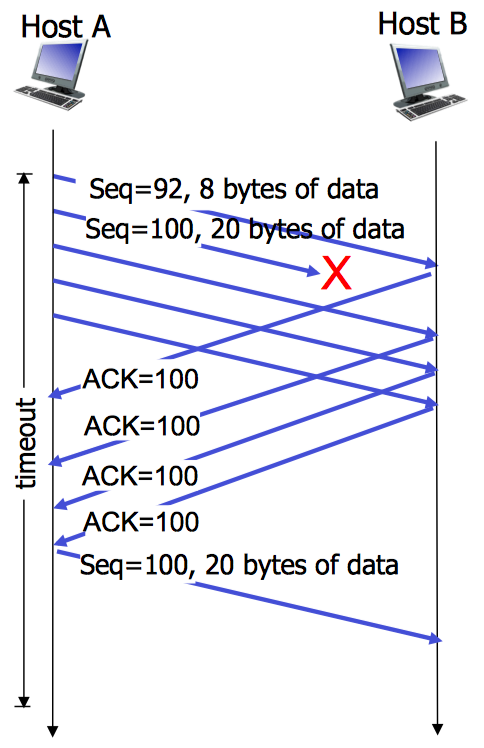
\includegraphics[width=5cm]{images/tcpfr.png}
  \caption{TCP Fast Retransmit}
  \label{fig:tcpfr}
\end{figure}

\paragraph{Handshaking} Come detto precedentemente questo protocollo prevede di stabilire la connessione prima di avviare la trasmissione in modo da accordarsi sui parametri di essa al fine di una corretta interpretazione dei dati.\\
Questo tipo di handshake prendere il nome di 3-way e prevede il seguente flusso (figura \ref{fig:syn}):
\begin{enumerate}
  \item \textbf{TX}: Invia TCP SYN msg con seq=x.
  \item \textbf{RX}: Risponde con seq=y, ACKbit=1 e \#ACK=x+1. (segnale server on)
  \item \textbf{TX}: Invia ACK di risposta al RX con \#ACK=y+1. (segnale client on)
\end{enumerate}
La chiusura della connessione invece prenvede anch'essa un ``botta e risposta'' di pacchetti ed ACK (\ref{fig:fin}):
\begin{enumerate}
  \item \textbf{TX}: Invia TCP FIN msg con seq=x.
  \item \textbf{RX}: Risponde con ACK per conferma di ricezione FIN ACKbit=1 e \#ACK=x+1.
  \item (in questa fase il client non può più inviare dati al server, mentre il server può ancora inviare dati)
  \item \textbf{RX}: Invia TCP FIN msg con seq=y.
  \item \textbf{TX}: Risponde con ACK per conferma di ricezione FIN ACKbit=1 e \#ACK=y+1.
\end{enumerate}
I due numeri x ed y sono numeri generati casualmente per questioni di sicurezza, difficilmente vedremo quindi sequenze partenti da zero (son Wireshark vedremo il numero relativo di sequenza di default).\\
Da questo momento in poi la connessione sarà terminata ed i due lati non potranno più comunicare fino a nuova connessione.

\begin{figure}[!hbpt]
  \centering
  \begin{minipage}{.45\textwidth}
    \centering
    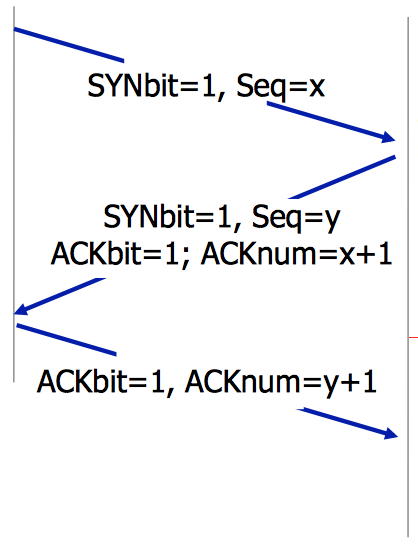
\includegraphics[width=\linewidth]{images/syn.png}
    \caption{Apertura connessione}
    \label{fig:syn}
  \end{minipage}\hfill
  \begin{minipage}{.45\textwidth}
    \centering
    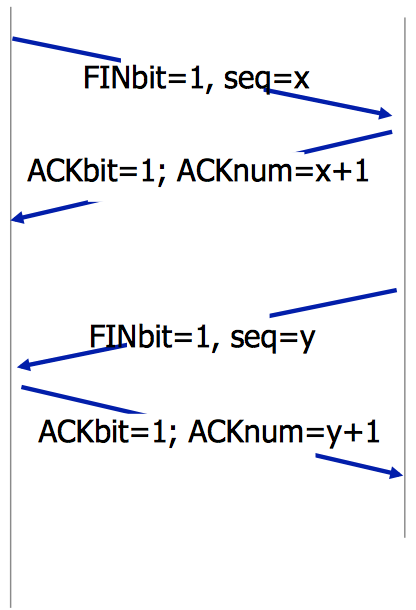
\includegraphics[width=\linewidth]{images/fin.png}
    \caption{Chiusura connessione}
    \label{fig:fin}
  \end{minipage}\hfill
\end{figure}

\paragraph{Congestionamento} TCP prevede il controllo del flusso di comunicazione. Inizialmente non era prevista la gestione, fu successivamente aggiunta la possibilità con ECN, il problema di utilizzo è dovuto al ritardo di introduzione per tanto si son preferite altre tecniche.\\
Ad oggi la gestione si basa sul dimensionamento delle finestra di ricezione nei due lati.
Lo stream di questo protocollo viene avviato a ``lentamente'' onde evitare di sovraccaricare il ricevitore e mano a mano alzerà la velocità, modificando il campo rwnd di ogni pacchetto TCP, con due tecniche:
\begin{itemize}
  \item \textbf{Additive Increase}: Aumenterà la dimensione della finestra di congestione (cwnd), ogni RTT, (di 1/cwnd ogni ACK ricevuto) fino alla rilevazione di una perdita.
  \item \textbf{Mutiplicative Decrease}: Dimezza la porta ogni perdita (conservativa).
\end{itemize}
In realtà il throughput sarà fissato dal min(cwnd, rwnd). Questo permette una migliore gestione adattata al traffico in reale in quel momento. Il rate di TCP si calcolerà con $rate=\frac{cwnd}{RTT}$. Spesso l'andamento è, dopo una fase di accellerazione, costante nel tempo perchè arrivo al massimo valore della finestra (limitato dalla rete). \\
Un'altra tecnica usata per la gestione del congestionamento è il \textbf{TCP Slow Start} dove il l'aumento del numero di pacchetti è esponenziale e non lineare come la tecnica precedente, aumentando la finestra di 1 MSS (1460 byte). In qualsiasi caso vi sarebbero moltissime soluzioni, per molti problemi, ma la scoglio più grande rimarrà comunque l'incapacità totale o quasi, per ethernet, di evolversi.

\paragraph{Perdita Pacchetto} Nel caso venga rilevata una perdita ci son due comportamenti, perdita rilevata con:
\begin{itemize}
  \item \textbf{Timeout}: Parto nuovamente da 1 MSS, cresco esponenzialmente fino alla soglia (metà del rate) e successivamente cresco linearmente.
  \item \textbf{Duplicate ACK}: Dimezzo la finestra e cresco linearmente.
\end{itemize}
E' molto più efficente quando rilevo per ACK duplicati (TCP Reno) piuttosto che da timeout (TCP Tahoe). Sono disponibili molte altre tecniche questo perchè sono dettagli di sola pertinenza lato sender.

\paragraph{Fairness} Il protocollo cerca di offrire a tutti quanti lo stesso servizio, senza privilegiarne nessuna, fornendo un rate=bandwidth/n.connessioni.


\section{Application Layer - LV5} \label{LV5} % 6 Gennaio 2017
\subsection{Introduzione}
Il livello applicativo è quello si può dire più vicino all'utente ed è costituito da tutto ciò che riguarda l'interazione con esso. Le applicazioni che fanno parte di questo livello son ad esempio le mail, il web, P2P, streaming video, ricerche, VOIP, ecc...\\
Le strutture con cui possono essere gestite queste applicazioni sono due, quella client-server, ovvero dove l'utente accede ad un server always on per scaricare/caricare le informazioni necessarie (Netflix), oppure quella P2P dove non esiste un server always on ma dove sono gli utenti finali stessi a comunicare tra di loro senza bisogno di strutture esterne (BitTorrent).

\subsection{Comunicazione}
La comunicazione su questo livello è strutturata a processi (client-server), il \textit{client process} sarà il processo che inizierà la comunicazione mentre il \textit{server process} sarà quello ad attendere di essere contattato dal client process.\\
Da qui si diramano moltissime tipologie, il messaggio può essere di risposta o di richiesta, devono essere definite le sintassi dei messaggi e la semantica, i protoccoli comunicativi (proprietari o no) ed altre numerose regole.\\
Questo layer prevede vengano garantiti alcuni servizi dai layer sottostanti come ad esempio:
\begin{itemize}
  \item \textbf{Data Integrity}: Transfert affidabili senza perdite.
  \item \textbf{Timing}: Bassi ritardi di comunicazione.
  \item \textbf{Throughput}: Richieste di banda minima o gestione elastica.
  \item \textbf{Security}: Integrità dei dati e criptografia.
\end{itemize}

\subsection{WEB e HTTP}

\subsection{FTP}

\subsection{Mail Exchange}

\subsection{P2P}





% \section{Ringraziamenti} Questo breve riepilogo non ha alcuno scopo se non quello di agevolare lo studio di me stesso, se vi fosse di aiuto siete liberi di usarlo. Le fonti su cui mi sono basato sono quelle relative al corso offerto (\textbf{Reti di Calcolatori (12CDUOA)}) dal Politecnico di Torino durante l'anno accademico 2016/2017.\\
% Non mi assumo nessuna responsabilità in merito ad errori o qualsiasi altra cosa. Fatene buon uso!

\bibliographystyle{abbrv}
\bibliography{simple}

\end{document}

% \begin{center}
% \begin{tabular}{ |c|c|c| }
%  \hline
%  Column1 & Column2 & Column3 \\
%  \hline
%  \hline
%  cell4 & cell5 & cell6 \\
%  \hline
%  cell7 & cell8 & cell9 \\
%  \hline
% \end{tabular}
% \end{center}
